\documentclass[11pt]{article}
\usepackage[margin=1in]{geometry}
\usepackage{volfit_preamble}
\graphicspath{{figures/}}

\title{\textbf{The LQD Model: Coordinates for the Space of Smiles}\\[2pt]
\large A density-first lecture on arbitrage-free volatility fitting\\[2pt]
\normalsize Vol-Fitter Technical Notes, No.~01}
\author{Vol-Fitter}
\date{\today}

\begin{document}
\maketitle

% Generated numbers.  lqd_tables.tex carries the shared production constants
% and the Jacobian timing table (gen_lqd.py); lqd_fresh_tables.tex the case
% files (gen_lqd_fresh.py); lqd_geometry_tables.tex the figures unique to this
% edition (gen_lqd_geometry.py).  Never retype a generated number.
% Auto-generated by Docs/notes/figures/gen_lqd.py — do not edit.
\newcommand{\lqdoptpts}{2001}
\newcommand{\lqdbarriercenter}{0.90}
\newcommand{\lqdbarrierscale}{50.0}
\newcommand{\lqdsviAL}{0.214458}
\newcommand{\lqdsviAR}{0.069023}
\newcommand{\lqdsvimu}{0.020613}
\newcommand{\lqdsvibetaL}{0.097073}
\newcommand{\lqdsvibetaR}{0.035757}
\newcommand{\lqdsvimaxerr}{0.23}
\newcommand{\lqdsvisigma}{20.62}
\newcommand{\lqdsviskew}{-0.3538}
\newcommand{\lqdsvicurv}{1.6474}
\newcommand{\lqdsvimart}{0.00e+00}
\newcommand{\lqdsvinfev}{7}
\newcommand{\lqdsvicoefftable}{\begin{tabular}{lr} \toprule Parameter & Value\\ \midrule $L$ & -1.87479110\\ $R$ & -3.08957252\\ $a_{2}$ & +0.38076853\\ $a_{3}$ & -0.04700855\\ $a_{4}$ & -0.00719617\\ $a_{5}$ & +0.00645578\\ $a_{6}$ & +0.00213226\\ \bottomrule \end{tabular}}
\newcommand{\lqddhmaxerr}{13.19}
\newcommand{\lqddhAL}{0.015341}
\newcommand{\lqddhAR}{0.014979}
\newcommand{\lqdtimingtable}{\begin{tabular}{rrrrrr} \toprule $N$ & $P$ & analytic (ms) & FD (ms) & speed-up & $|\Delta\mathrm{cost}|$\\ \midrule 6 & 7 & 15.3 & 25.0 & 1.64$\times$ & 5.6e-20\\ 8 & 9 & 20.9 & 29.2 & 1.40$\times$ & 1.4e-19\\ 10 & 11 & 26.6 & 41.7 & 1.57$\times$ & 8.9e-20\\ 12 & 13 & 27.3 & 47.0 & 1.72$\times$ & 2.0e-20\\ \bottomrule \end{tabular}}

% Auto-generated by Docs/notes/figures/gen_lqd_fresh.py -- do not edit.
% Exact-20%-ATM half-year logistic toy.
\newcommand{\lqdfreshtoyexpiry}{0.50}
\newcommand{\lqdfreshtoyatm}{20.0000}
\newcommand{\lqdfreshtoyscale}{0.08125025}
\newcommand{\lqdfreshtoymu}{-0.01088288}
\newcommand{\lqdfreshtoyuatm}{0.533436}
\newcommand{\lqdfreshtoyuatmpct}{53.3436}
\newcommand{\lqdfreshtoyuten}{0.796524}
\newcommand{\lqdfreshtoystriketen}{1.105171}
\newcommand{\lqdfreshtoyshareten}{0.24722094}
\newcommand{\lqdfreshtoycashten}{0.22487593}
\newcommand{\lqdfreshtoycallten}{0.02234501}
\newcommand{\lqdfreshtoycalltenpct}{2.2345}
\newcommand{\lqdfreshtoyivten}{20.5977}
% SPX-like production fit.
\newcommand{\lqdfreshspxorder}{9}
\newcommand{\lqdfreshspxnquotes}{24}
\newcommand{\lqdfreshspxatm}{21.7961}
\newcommand{\lqdfreshspxskew}{-0.177846}
\newcommand{\lqdfreshspxcurvature}{0.002673}
\newcommand{\lqdfreshspxmaxerr}{1.341}
\newcommand{\lqdfreshspxrmserr}{0.408}
\newcommand{\lqdfreshspxnfev}{8}
\newcommand{\lqdfreshspxAL}{0.157473}
\newcommand{\lqdfreshspxAR}{0.037786}
\newcommand{\lqdfreshspxbetaL}{0.073087}
\newcommand{\lqdfreshspxbetaR}{0.019259}
\newcommand{\lqdfreshspxvarswap}{22.9685}
\newcommand{\lqdfreshspxmart}{\ensuremath{-1.11\times10^{-16}}}
% Asymmetric double-hat event fit.
\newcommand{\lqdfresheventorder}{16}
\newcommand{\lqdfresheventnquotes}{37}
\newcommand{\lqdfresheventweightleft}{56.0}
\newcommand{\lqdfresheventmeanleft}{-0.074804}
\newcommand{\lqdfresheventmeanright}{0.085196}
\newcommand{\lqdfresheventmaxerr}{2.444}
\newcommand{\lqdfresheventrmserr}{0.999}
\newcommand{\lqdfresheventAL}{0.015531}
\newcommand{\lqdfresheventAR}{0.014044}
\newcommand{\lqdfresheventmart}{\ensuremath{-2.22\times10^{-16}}}
\newcommand{\lqdfresheventmaxquotediv}{2.444}
% Convexity and derivative checks.
\newcommand{\lqdfreshminbutterfly}{0.224428}
\newcommand{\lqdfreshbutterflyrelerr}{0.0182}
\newcommand{\lqdfreshjacnparams}{10}
\newcommand{\lqdfreshjacmaxrel}{\ensuremath{2.88\times10^{-5}}}
% Ready-to-drop worked-example tables.
\newcommand{\lqdfreshtoytable}{%
\begin{tabular}{lr}
\toprule
Quantity & Production value\\
\midrule
Solved scale & 0.08125025\\
Martingale shift & -0.01088288\\
ATM percentile & 53.3436\%\\
$C(0.10)$ & 0.02234501\\
$\sigma_{\mathrm{BS}}(0.10)$ & 20.5977\%\\
\bottomrule
\end{tabular}}
\newcommand{\lqdfreshfitdiagtable}{%
\begin{tabular}{lrr}
\toprule
Diagnostic & SPX-like & Event\\
\midrule
Model order & 9 & 16\\
Quotes & 24 & 37\\
Max error (vol bp) & 1.341 & 2.444\\
RMS error (vol bp) & 0.408 & 0.999\\
$A_L$ & 0.157473 & 0.015531\\
$A_R$ & 0.037786 & 0.014044\\
\bottomrule
\end{tabular}}

% Auto-generated by Docs/notes/figures/gen_lqd_geometry.py -- do not edit.
\newcommand{\lqdgeomnshape}{7}
\newcommand{\lqdgeomshapedriftsigma}{2.17}
\newcommand{\lqdgeomshapedriftskew}{\ensuremath{7.88\times10^{-5}}}
\newcommand{\lqdgeomshapedriftcurv}{\ensuremath{6.27\times10^{-3}}}
\newcommand{\lqdgeomshapewingmove}{103}
\newcommand{\lqdgeomshapeatmmove}{2.17}
\newcommand{\lqdgeomretargetresid}{\ensuremath{6.00\times10^{-14}}}
\newcommand{\lqdgeomskewbump}{0.04}
\newcommand{\lqdgeommingaplegit}{0.00087}
\newcommand{\lqdgeommingapcross}{-0.00218}
\newcommand{\lqdgeomugapcross}{0.39}
\newcommand{\lqdgeommingaphealed}{\ensuremath{-3.45\times10^{-6}}}
\newcommand{\lqdgeomchartsmart}{\ensuremath{1.11\times10^{-16}}}
\newcommand{\lqdgeomjacnparams}{10}
\newcommand{\lqdgeomjacmaxrel}{\ensuremath{2.88\times10^{-5}}}


\begin{abstract}
A volatility smile is a probability distribution seen through the Black
formula.  Most fitters nevertheless parametrize the smile directly and then
police, with penalties, the awkward nonlinear conditions under which their
curve still corresponds to a genuine distribution.  This lecture develops the
Vol-Fitter's \emph{LQD} (log-quantile-density) model the other way around, as
the answer to a coordinate problem: among all the charts one can draw on the
space of arbitrage-free slices --- price, implied volatility, distribution
function, density, quantile --- find the one in which that space becomes
\emph{all of coordinate space}, so that the optimizer can roam freely and
every point it visits already prices from a genuine law.  The answer is to
model the logarithm of the quantile density of the log-forward return as two
universal boundary terms plus a Legendre expansion,
$\log q(u) = -\log u - \log(1-u) + g(u)$.  Positivity of the density is then
structural, a single scalar shift enforces the martingale condition, and the
two endpoint values of $g$ identify both the last finite moments of the
distribution and its Lee wing slopes; the only genuine constraint that
survives is one inequality, $A_R<1$, the price of a finite forward.  From this
construction we derive pricing as one cumulative integral, exact closed-form
ATM level/skew/curvature handles with an orthogonal chart around them, the
calibration objective, an analytic residual Jacobian obtained from a clean
cancellation identity, and soft convex-order control across expiries --- read
off the same upper-share ledger that prices the calls.  Every figure is
generated by the production calibrator on deterministic synthetic
benchmarks: a ten-parameter fit to an SPX-like strip reaches a maximum error
of \lqdfreshspxmaxerr\ volatility basis points, and a seventeen-parameter fit
recovers an asymmetric bimodal event density to \lqdfresheventmaxerr\ vol
basis points.  Market-fit evidence lives in the backtest reports; what this
lecture establishes is the machine itself.
\end{abstract}

\tableofcontents
\newpage

%======================================================================
\section{The shape of the problem}
\label{sec:problem}

Here is a failure mode every production smile fitter meets.  You parametrize
implied volatility with some pleasant curve, fit seven liquid strikes, and the
residuals look excellent.  Then a risk system differentiates your curve twice
--- because the second strike derivative of a call \emph{is} the risk-neutral
density, as we recall below --- and finds it negative between two quotes.
Your smooth, well-fitting smile is quoting a butterfly you would pay to be
lifted on: free money for the counterparty, a phantom probability of
$-2\%$ for the risk report.  Nothing in the fit was wrong numerically.  The
parametrization simply did not know that a smile is not free to be any curve.

The standard remedy is to keep the pleasant curve and add penalties: evaluate
the density (or its proxy) on a grid, punish negativity, and hope the
optimizer lands inside the feasible set.  This works, mostly, but it has a
characteristic cost profile.  The constraint is \emph{global} and
\emph{nonlinear} in the parameters, so it must be re-checked at every strike
and every iterate; the optimizer spends its time crawling along the boundary
of the feasible set, exactly where the penalty gradients fight the data
gradients; and when the market is sparse or stressed --- precisely when you
most need the fitter --- the boundary is where the solution wants to live.

The LQD model spends none of that effort, because it asks a different
question first.

\begin{quote}
\emph{The set of arbitrage-free slices is a well-defined mathematical object.
In which coordinates is that set trivial --- all of coordinate space, no
boundary, nothing to police?}
\end{quote}

This lecture is the answer worked out in full, and the sense in which it is a
lecture is worth one sentence: we will build the model from first principles,
prove the small number of facts that carry it, and keep the numerical
plumbing in clearly marked asides, so that a reader who knows the Black
formula and one year of probability can reconstruct everything.  The
destination is fixed by production, and it is protected by the following
invariants.

\begin{invariant}
\begin{enumerate}[leftmargin=1.6em]
\item Every admissible parameter vector prices from a genuine non-negative
density: butterfly-freedom is structural, never a penalty
(\cref{prop:nobutterfly}).
\item The only hard admissibility condition is the single inequality $A_R<1$
--- a finite forward --- guarded by a smooth barrier before the wall
(\cref{sec:tails,sec:calib}).
\item The martingale normalization is one scalar shift; it changes neither
the density's shape, nor its tails, nor its positivity (\cref{sec:pricing}).
\item The ATM handles $(\sigma_0,s_0,\kappa_0)$ are exact closed-form
functionals of the slice --- the same three coordinates the graph
extrapolator of Note~14 propagates (\cref{sec:handles}).
\end{enumerate}
\end{invariant}

\paragraph{A running example.}  Lectures profit from a recurring character.
Ours is a deterministic, SPX-like strip of \lqdfreshspxnquotes\ quotes at the
expiry $\tau=0.75$, sampled from a skewed SSVI-shaped curve
(\cref{app:oracles}) with a reproducible sub-two-basis-point microstructure
ripple, and fitted \emph{once} by the production calibrator with a
nine-mode LQD slice.  Almost every figure in this note draws that one fitted
slice from a different angle; its full case file, with numbers, is
\cref{sec:case_spx}.  A second character --- a bimodal event distribution ---
appears when we need to stress the basis (\cref{sec:case_event}).

\paragraph{What this note is not.}  The examples are \emph{synthetic
approximation benchmarks}: they measure how well the parametrization can
reproduce a known clean curve, not how well it fits noisy market quotes.
Market-fit evidence --- RMS against bid--ask NBBO quotes, in and out of
sample, against an SVI-JW baseline --- lives in the backtest harness
(\texttt{backend/backtest/}) and its reports.

%======================================================================
\section{What a smile really is}
\label{sec:slice}

\subsection{Normalized units, and the three clocks}

Fix one expiry.  All the securities we price are functions of the terminal
spot $S$, and everything deterministic --- discounting, forwards, carry ---
can be divided out before modelling begins.  We therefore work with the
\emph{log-forward return}
\begin{equation}
X=\log\frac{S}{F},
\qquad Y=e^{X}=\frac{S}{F},
\label{eq:X_def}
\end{equation}
with $F$ the forward to the expiry, under the forward measure of that expiry.
Strikes are quoted in log-moneyness $k=\log(K/F)$, and the \emph{normalized
call} is
\begin{equation}
C(k)=\E\!\left[(e^{X}-e^{k})^{+}\right],
\qquad \E[e^{X}]=1,
\label{eq:call_def}
\end{equation}
where the second equality --- the martingale, or forward, condition --- says
that the forward really is the mean of the terminal spot.  A dollar quote
$C^{\$}$ converts to these units by $C=C^{\$}/(DF)$ with $D$ the discount
factor; nothing else about rates or carry will appear again.  Deterministic
carry is a standing assumption of the whole note; it is what legitimizes
working slice by slice under each expiry's forward measure, and it is
revisited when slices are coupled in \cref{sec:calendar}.

One symbol of time is enough, but it must be the right one.  Production
distinguishes the \emph{expiry date} from its \emph{calendar year fraction}
and from the \emph{active variance time} --- calendar time dilated by
scheduled events (Note~11).  Everything in this note that multiplies a
variance, scales a vega, or annualizes a handle uses the active time, written
\begin{equation}
\tau \;=\; \text{active variance time to expiry}
\qquad(\text{the calibrator's \texttt{prepared.tau}}),
\end{equation}
which equals the calendar fraction whenever the event clock is off.  Total
implied variance at log-moneyness $k$ is $w(k)=\sigma^{2}(k)\,\tau$, with
$\sigma$ the Black implied volatility.  A \emph{volatility basis point}
(vol bp) is $10^{-4}$ in volatility.  When several expiries appear at once we
index them $\tau_1<\tau_2<\cdots$; a single unlabelled slice is always ``the''
expiry.

\subsection{Breeden--Litzenberger, and the slice as a law}

The reason a smile cannot be an arbitrary curve is one integration by parts
away.  Write the call as a function of the normalized strike $y=e^{k}$; when
$Y$ has a density $f_Y$,
\begin{equation}
\frac{\partial C}{\partial y}=-\,\Prob(Y>y),
\qquad
\frac{\partial^{2} C}{\partial y^{2}}=f_Y(y)\;\ge\;0 .
\label{eq:BL}
\end{equation}
This is the Breeden--Litzenberger identity \cite{BreedenLitzenberger1978}:
the call curve determines the distribution, and conversely every property of
the call curve that a static portfolio can monetize is a property of the
distribution.  A \emph{butterfly} --- long one call at $y-h$, long one at
$y+h$, short two at $y$ --- costs $C(y-h)-2C(y)+C(y+h)$, and by
\eqref{eq:BL} its price per $h^{2}$ converges to the density at $y$.  A
negative butterfly price is exactly a negative density.

\begin{definition}[Arbitrage-free slice]
\label{def:slice}
A \emph{slice} is a call curve $C(k)$ of the form \eqref{eq:call_def} for
some law of $X$ with $\E[e^{X}]=1$.  Equivalently (for laws with a density):
$C$ is decreasing and convex in the strike $y=e^{k}$, with $C\to1$ as
$y\to0$ and $C\to0$ as $y\to\infty$, and slope $\ge-1$.
\end{definition}

The space of slices, then, is really the space of mean-one probability laws
on $(0,\infty)$.  That is the object we must parametrize, and
\cref{fig:butterfly} shows our running example wearing both descriptions at
once: a convex call curve on the left, and on the right the density recovered
by pricing actual finite-width butterflies on the fitted slice.

\begin{figure}[H]
\centering
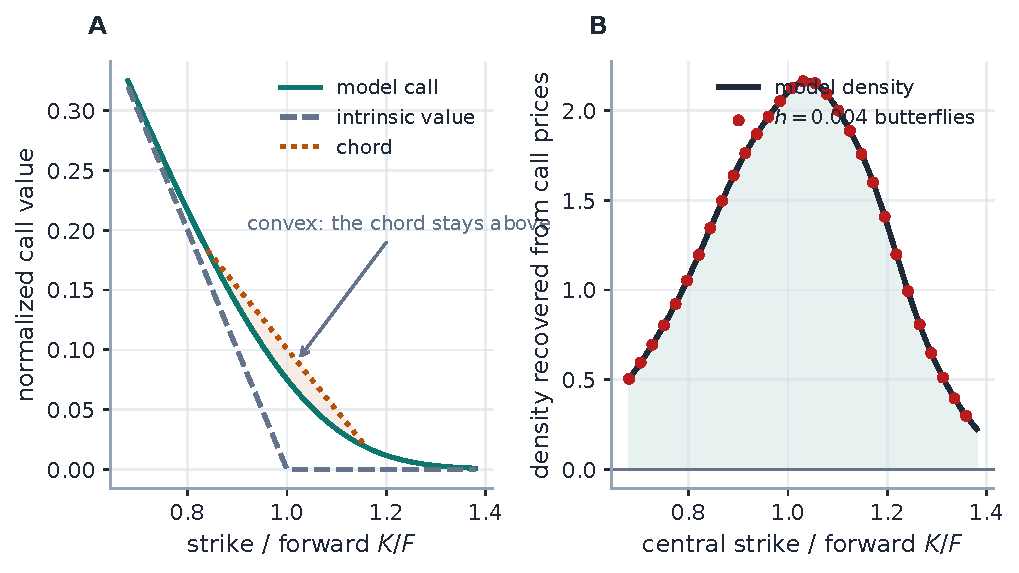
\includegraphics[width=\textwidth]{fig_lqd_fresh_butterfly.pdf}
\caption{The running SPX-like fit as a tradable object.  Panel A: the
normalized call curve is decreasing and convex --- every chord sits above the
curve, so every butterfly has non-negative price.  Panel B: discrete
butterflies of half-width $h=0.004$, priced off the fitted slice and divided
by $h^{2}$, recover the model density to a relative
\lqdfreshbutterflyrelerr\ (the minimum butterfly value on the grid is
$\lqdfreshminbutterfly>0$).  Butterfly-freedom is not something this fit
achieved; it is something the parametrization cannot lose.}
\label{fig:butterfly}
\end{figure}

\subsection{The notation ledger}

Because this lecture insists on few symbols, here they all are.  Each is
defined again where it first works for a living; none is ever reused with a
second meaning.

\begin{table}[H]
\centering\footnotesize
\setlength{\tabcolsep}{4pt}
\begin{tabular}{@{}llll@{}}
\toprule
$X,\ Y=e^{X}$ & log-forward return, gross return &
$u,\ z=\log\frac{u}{1-u}$ & rank (percentile), log-odds\\[2pt]
$k,\ C(k),\ P(k)$ & log-moneyness; call, put &
$Q,\ q=Q'$ & quantile of $X$; quantile density\\[2pt]
$w,\ \sigma,\ \tau$ & total variance $\sigma^{2}\tau$; vol; active time &
$g,\ \theta$ & smooth part of $\log q$; coefficients\\[2pt]
$\Black(k,w)$ & normalized Black call &
$A_L,\ A_R$ & endpoint (tail) scales $e^{g(0)},e^{g(1)}$\\[2pt]
$\mu$ & martingale shift &
$G$ & upper share $\int e^{Q}$ above a rank\\[2pt]
$\sigma_0,\ s_0,\ \kappa_0$ & ATM vol, skew, curvature &
$\beta,\ \psi,\ p$ & Lee slope, Lee map, moment order\\[2pt]
$\lambda,r;\ c,\gamma$ & ridge; barrier centre/steepness &
$H,J,U,V,\alpha,\xi$ & the ATM-orthogonal chart\\
\bottomrule
\end{tabular}
\caption{Every symbol in the note.  $\PhiN$ and $\phin$ are the standard
normal CDF and PDF.  One differentiation convention holds throughout: a
\emph{prime} is the derivative of a function of one variable ($C'$, $w'$,
$\sigma'$); a \emph{subscripted} $\partial$ is a partial derivative of a
function of several ($\partial_k\Black$, $\partial G/\partial\theta$).
Symbols local to one appendix (the SSVI oracle's $\vartheta,\rho,\phi$) stay
in that appendix.}
\label{tab:ledger}
\end{table}

%======================================================================
\section{Six charts for one space}
\label{sec:charts}

We are hunting for coordinates on the space of mean-one laws.  A good way to
appreciate the answer is to price the alternatives first --- this is a
shopping trip, and the currency is \emph{constraints left over}.

\paragraph{The price chart.}  Parametrize $C(k)$ itself.  The constraint set
\cref{def:slice} is a convex cone with curved walls: monotonicity and
convexity at \emph{every} strike, plus the endpoint conditions.  Convexity of
a parametric curve is a global condition on second derivatives; enforcing it
for a flexible family means a grid of inequality constraints.  Nothing is
free.

\paragraph{The volatility chart.}  Parametrize $\sigma(k)$ --- what every
trader quotes, and what SVI does.  The density is now a \emph{nonlinear}
second-order differential expression in $w(k)=\sigma^{2}(k)\tau$ (Gatheral's
$g$-function \cite{Gatheral2006,GatheralJacquier2014}); non-negativity is an
implicit, parameter-global boundary that no useful family satisfies
identically.  This chart is the most convenient to \emph{quote} and the most
expensive to \emph{police} --- the note's opening failure mode lives here.

\paragraph{The distribution chart.}  Parametrize the CDF $F_X$.  One
constraint survives: monotonicity, again at every point.  Closer.

\paragraph{The density chart.}  Parametrize $f_X\ge0$ directly.  Positivity
of a flexible parametric curve is still a pointwise constraint (unless one
squares or exponentiates, of which more below), and two integral constraints
remain: total mass one, and the martingale $\int e^{x}f_X(x)\,\dd x=1$.

\paragraph{The quantile chart.}  Parametrize the quantile function
$Q=F_X^{-1}$ on the rank $u\in(0,1)$.  One constraint: $Q$ strictly
increasing.  And here the structure finally cooperates, because monotonicity
--- unlike convexity or positivity-of-a-difference --- is destroyed by
\emph{one} derivative, not two.

\paragraph{The free chart.}  Let $q(u)=Q'(u)$ be the \emph{quantile density}.
Then $Q$ increasing $\iff q>0$ $\iff \log q$ is \emph{any} real function.
Modelling $\log q$ removes the last pointwise constraint; what remains are
one integrability condition (so that the martingale integral converges) and
one scalar normalization (to set its value to one) --- and, remarkably, we
will see in \cref{sec:tails,sec:pricing} that these cost a single inequality
and a single additive shift.  \Cref{tab:charts} tallies the trip, and
\cref{fig:charts} shows the same fitted slice in four of the charts: the
constraints that are visibly at work in the first three panels are simply
\emph{absent} in the fourth.

\begin{table}[H]
\centering\small
\begin{tabular}{@{}llll@{}}
\toprule
Chart & Object & Constraints left over & Type\\
\midrule
Price & $C(k)$ & decreasing, convex, endpoints & pointwise, global\\
Volatility & $\sigma(k)$ & $f\ge0$ as a nonlinear ODE expression &
implicit, global\\
Distribution & $F_X$ & increasing & pointwise\\
Density & $f_X$ & $f\ge0$; mass $=1$; $\E[e^{X}]=1$ & pointwise $+$ 2
integrals\\
Quantile & $Q(u)$ & increasing & pointwise\\
Log quantile density & $\log q(u)$ & $A_R<1$; one scalar shift & \emph{one
inequality}\\
\bottomrule
\end{tabular}
\caption{The shopping trip.  Each chart describes the same space of mean-one
laws; only the last reduces its boundary to a single scalar inequality, with
the normalization absorbed by a shift rather than a constraint.}
\label{tab:charts}
\end{table}

\begin{figure}[H]
\centering
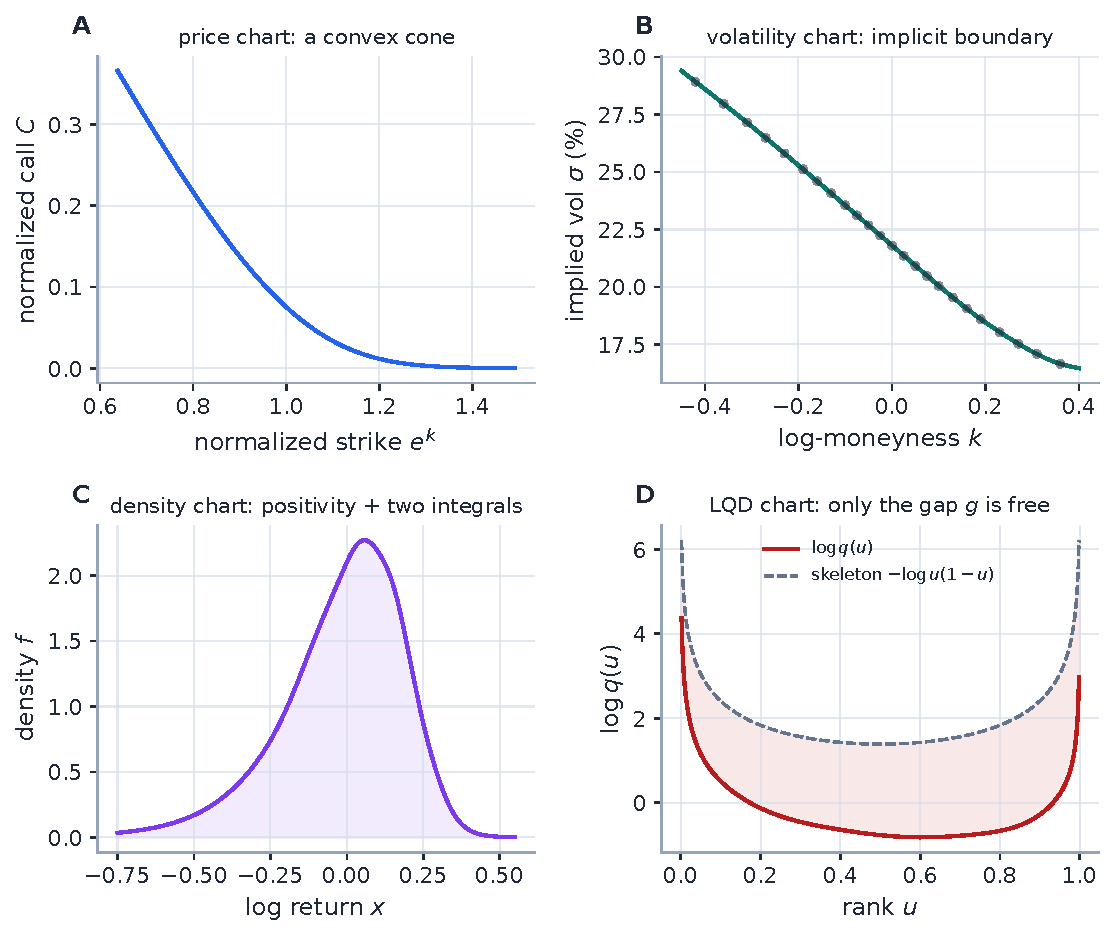
\includegraphics[width=0.94\textwidth]{fig_lqd_geom_charts.pdf}
\caption{One fitted slice --- the running SPX-like example --- in four
coordinate charts.  A: the price chart, where no-arbitrage is a convex cone.
B: the volatility chart, where it is an implicit nonlinear boundary (the
quotes ride the fitted curve).  C: the density chart, where it is positivity
plus two integral constraints.  D: the LQD chart of \cref{def:lqd}: the
classical U of $\log q$, diving to $+\infty$ at both ends along the
universal skeleton $-\log u-\log(1-u)$ (dashed).  The skeleton is the same
for every slice; the model's entire freedom is the shaded gap $g$ between
the two curves, and \emph{any} smooth gap --- shifted, bent, or oscillating
--- is another arbitrage-free slice, provided only that the single
inequality $A_R<1$ holds at the right edge.  The fit's martingale check is
$|\E[e^{X}]-1|=\lqdgeomchartsmart$.}
\label{fig:charts}
\end{figure}

\subsection{The model in one equation}

It remains to choose a basis for $\log q$, and the choice is forced by two
requirements: the tails must be \emph{right by construction} (next section),
and the body must be flexible, well-conditioned, and cheap.  The LQD answer
splits $\log q$ into a universal singular skeleton and a smooth part:

\begin{definition}[The LQD slice]
\label{def:lqd}
Fix an order $N\ge4$ and coefficients $\theta=(L,R,a_2,\dots,a_N)$.  The LQD
quantile density is
\begin{equation}
\boxed{\;
q(u)=\frac{e^{g(u)}}{u\,(1-u)},
\qquad
g(u)=(1-u)\,L+u\,R+\sum_{n=2}^{N}a_n\,P_n(1-2u),
\;}
\label{eq:lqd_main}
\end{equation}
for $u\in(0,1)$, with $P_n$ the Legendre polynomials.  The quantile is
$Q(u)=\mu+\int_{1/2}^{u}q$, with the scalar $\mu$ fixed by the martingale
condition $\E[e^{X}]=\int_0^1 e^{Q(u)}\dd u=1$.
\end{definition}

Equivalently $\log q(u)=-\log u-\log(1-u)+g(u)$: the two logarithmic terms
are the skeleton, the smooth $g$ is everything else.  The shipped default
$N=6$ carries seven parameters; the API accepts $4\le N\le16$, and higher $N$
adds body detail without ever touching the no-arbitrage mechanism.  Inverting
$q=1/f_X(Q)$ gives the density at the rank $u$:
\begin{equation}
f_X\big(Q(u)\big)=\frac{1}{q(u)}=u\,(1-u)\,e^{-g(u)}\;\ge\;0
\qquad\text{for every }\theta ,
\label{eq:density}
\end{equation}
and this single line is the whole no-arbitrage mechanism.  In code:

\begin{lstlisting}[caption={The LQD density is structurally non-negative ---
no constraint, no penalty (distilled from
\texttt{models/lqd/quadrature.py}).},label={lst:lqd_density}]
def density(u, g):        # g(u) = (1-u) L + u R + sum a_n P_n(1-2u)
    return u * (1 - u) * np.exp(-g)   # >= 0 for ANY g: no butterfly
\end{lstlisting}

\begin{proposition}[A single LQD slice is butterfly-free]
\label{prop:nobutterfly}
Suppose $q>0$ on $(0,1)$ and the martingale integral $\int_0^1 e^{Q(u)}\dd u$
is finite.  After the scalar shift of $Q$ that makes this integral one, the
call curve $C(k)=\int_{u_k}^{1}(e^{Q(u)}-e^{k})\,\dd u$, with $u_k$ the rank
where $Q(u_k)=k$, is generated by a mean-one probability law on $Y>0$: the
slice is free of butterfly arbitrage, and put--call parity
$C(k)-P(k)=1-e^{k}$ holds identically.
\end{proposition}

\begin{proof}
Since $q>0$, $Q$ is strictly increasing and is the quantile of a genuine law
for $X$; then $Y=e^{X}>0$ and the shift enforces $\E[Y]=1$.  The displayed
$C(k)$ is just $\E[(Y-e^{k})^{+}]$ written rank-by-rank ($u$ is a uniform
variable and $Y=e^{Q(u)}$), so monotonicity and convexity in strike follow
from \eqref{eq:BL}; the put integral
$P(k)=\int_0^{u_k}(e^{k}-e^{Q(u)})\,\dd u$ subtracts to
$C-P=\int_0^1(e^{Q}-e^{k})=1-e^{k}$.  No positivity inequality is ever
checked.
\end{proof}

\begin{heuristic}
Why does the quantile side succeed where the density side struggled?  Because
exponentiating kills a \emph{pointwise} constraint but not an \emph{integral}
one.  On the density side, $f=e^{\phi}$ buys positivity but leaves two
integral constraints ($\int f=1$, $\int e^{x}f=1$) coupling all parameters
nonlinearly.  On the quantile side, $q=e^{\ell}$ buys monotonicity, the mass
constraint is \emph{automatic} (every increasing $Q$ on $(0,1)$ is a quantile
--- ranks are born normalized), and the one remaining integral constraint is
solved, not imposed: shifting $Q$ by a constant multiplies $\E[e^{X}]$ by
$e^{\mu}$, so one scalar $\mu$ absorbs it exactly, leaving the shape of the
law untouched.  One chart, zero pointwise constraints, zero residual
equality constraints.
\end{heuristic}

\paragraph{Why this is the right trade.}  A direct-volatility model spends
optimizer effort policing arbitrage; the LQD model spends none, because the
feasible set \emph{is} the set of laws.  The price is two scalar
nonlinearities --- the shift $\mu$ (one logarithm of one integral,
\cref{sec:pricing}) and the tail admissibility $A_R<1$ (\cref{sec:tails})
--- both imposed once per residual evaluation, not at every quote.

%======================================================================
\section{Tails first: the endpoint skeleton}
\label{sec:tails}

A basis for $g$ should be chosen tails-first, because extrapolation is where
smile models die.  The far wings of a slice are constrained by a classical
and completely model-free result, Lee's moment formula \cite{Lee2004}, and
the two logarithmic terms in \eqref{eq:lqd_main} are engineered so that LQD
lands \emph{inside} Lee's bounds automatically, with the wing slopes carried
by two readable parameters.  This section owns that story; the cross-model
treatment of wings is Note~09's.

\subsection{Endpoint scales are quantile slopes}

The skeleton terms diverge at the ranks' endpoints, and the smooth part $g$
decides \emph{how fast}.  Because $P_n(1)=1$ and $P_n(-1)=(-1)^{n}$, the two
endpoint values of $g$ are
\begin{equation}
A_L:=e^{g(0)}=\exp\Big(L+\sum_{n\ge2}a_n\Big),
\qquad
A_R:=e^{g(1)}=\exp\Big(R+\sum_{n\ge2}(-1)^{n}a_n\Big).
\label{eq:endpoint_scales}
\end{equation}
Their meaning is best read in the log-odds coordinate $z=\log\frac{u}{1-u}$
that will run the whole pricing machine.  Since (writing $u(z)$ for the
inverse map $u=1/(1+e^{-z})$, whose derivative is $u(1-u)$)
\begin{equation}
\frac{\dd Q}{\dd z}=q(u)\,u(1-u)=e^{g(u(z))},
\label{eq:q_logit}
\end{equation}
the quantile has \emph{finite slope} $e^{g}$ in $z$ everywhere, and at the
two ends
\begin{equation}
Q(z)=\mu+A_L\,z+O(1)\ \ (z\to-\infty),
\qquad
Q(z)=\mu+A_R\,z+O(1)\ \ (z\to+\infty).
\end{equation}
So $A_L$ and $A_R$ are the asymptotic speeds at which log-return quantiles
recede per unit of log-odds: genuine tail \emph{scales}, not diagnostics.

\subsection{Exponential tails, the moment strip, and the one hard wall}

Linear quantiles in log-odds mean exponential tails in return space.  To see
it, ask how much probability lives above the return level $x=Q(z)$: exactly
the rank remainder $1-u(z)$, which behaves like $e^{-z}$ for large $z$.
Inverting the asymptote $x\approx\mu+A_Rz$ gives $z\approx(x-\mu)/A_R$, so
\begin{equation}
\Prob(X>x)\asymp e^{-x/A_R}\quad(x\to+\infty),
\qquad
\Prob(X<x)\asymp e^{\,x/A_L}\quad(x\to-\infty):
\label{eq:exp_tails}
\end{equation}
each tail is exponential, with decay rate the reciprocal of its scale.

Moments now follow from a single change of variables, and it is worth doing
once slowly because the whole admissibility story drops out.  Any
expectation is a rank integral, and in log-odds the rank measure carries an
intrinsic tent-shaped weight:
\begin{equation}
\E\big[h(X)\big]
=\int_0^1 h\big(Q(u)\big)\,\dd u
=\int_{-\infty}^{\infty}h\big(Q(z)\big)\,
\underbrace{u(z)\big(1-u(z)\big)}_{\;\asymp\;e^{-|z|}}\,\dd z .
\label{eq:rank_integral}
\end{equation}
Take $h(x)=e^{rx}$.  On the right, $e^{rQ(z)}\asymp e^{rA_Rz}$ against the
weight $e^{-z}$: the integrand behaves like $e^{(rA_R-1)z}$, integrable at
$+\infty$ iff $rA_R<1$.  On the left, $e^{rQ(z)}\asymp e^{rA_Lz}$ against
the weight $e^{+z}$: the integrand behaves like $e^{(rA_L+1)z}$, integrable
at $-\infty$ iff $rA_L>-1$.  So $\E[e^{rX}]$ converges precisely on the
strip
\begin{equation}
-\frac{1}{A_L}<r<\frac{1}{A_R}\,,
\end{equation}
each endpoint lost exactly when the exponential growth of $e^{rQ}$ ties the
exponential decay of the weight.  In return moments --- recalling
$Y=e^{X}$ --- the strip says that the last finite moments are
\begin{equation}
p_R^{*}=\sup\{p\ge0:\E[Y^{1+p}]<\infty\}=\frac{1}{A_R}-1,
\qquad
p_L^{*}=\sup\{p\ge0:\E[Y^{-p}]<\infty\}=\frac{1}{A_L}.
\label{eq:critical}
\end{equation}
One point of the strip is load-bearing.  The martingale integral
$\E[e^{X}]$ is the case $r=1$, and $r=1$ lies inside the strip iff
\begin{equation}
A_R<1
\qquad\text{(finite forward)}
\label{eq:AR_wall}
\end{equation}
--- the single wall promised in \cref{tab:charts}.  No left-hand condition
exists because $r=1>-1/A_L$ always.  The wall is not an artefact of the
basis: any law whose right return tail is exponential with scale $\ge1$ has
an infinite mean, whatever model writes it down.

\begin{caution}
$A_R<1$ is a genuine hard constraint, not a regularization preference: a
parameter vector with $A_R\ge1$ assigns the forward an \emph{infinite} mean,
and its ``prices'' are meaningless.  The calibrator enforces it twice ---
a hard rejection at $A_R\ge1-\eps_R$ and a smooth softplus barrier that
engages well before the wall (\cref{sec:calib}) --- so both the analytic and
the finite-difference Jacobians stay smooth as the optimizer approaches the
boundary.  Fits that live near the wall should be treated as fragile even
when admissible (\cref{sec:limits}).
\end{caution}

\subsection{From moments to Lee slopes}

Lee's moment formula turns \eqref{eq:critical} into wing geometry.  Writing
$\beta_R=\limsup_{k\to+\infty}w(k)/k$ and
$\beta_L=\limsup_{k\to-\infty}w(k)/|k|$ for the asymptotic slopes of total
implied variance, Lee proved
\begin{equation}
\beta=\psi(p),
\qquad
\psi(p)=2-4\big(\sqrt{p^{2}+p}-p\big)\in(0,2],
\label{eq:lee_psi}
\end{equation}
with $p$ the relevant critical exponent from \eqref{eq:critical}.  For LQD,
\begin{equation}
\beta_L=\psi\!\Big(\frac{1}{A_L}\Big),
\qquad
\beta_R=\psi\!\Big(\frac{1}{A_R}-1\Big),
\qquad A_R<1 .
\label{eq:lee_slopes}
\end{equation}
The endpoint coefficients therefore do double duty: they regularize
extrapolation \emph{and} identify the moment budget and the Lee-consistent
wing slopes.  A calibration may fit $L,R$ freely (subject only to the wall)
or impose explicit wing priors by pinning $A_L,A_R$ through
\eqref{eq:endpoint_scales}.  \Cref{fig:tailmap} draws the two maps.

\begin{figure}[H]
\centering
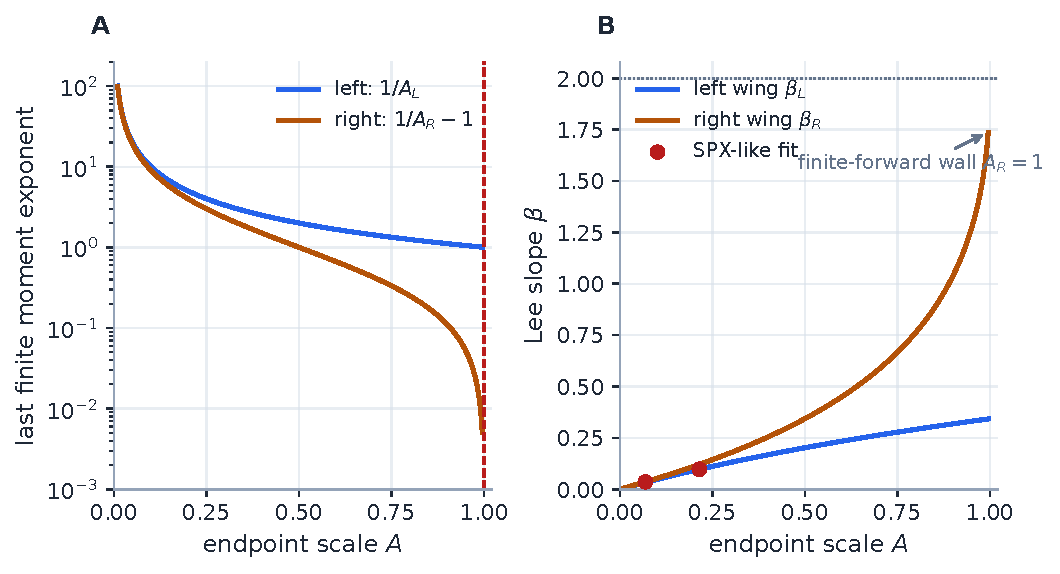
\includegraphics[width=\textwidth]{fig_lqd_tail_map.pdf}
\caption{The tail dial.  Panel A: the last finite moment exponent as a
function of the endpoint scale, $1/A_L$ on the left tail and $1/A_R-1$ on the
right; the dashed line is the finite-forward wall $A_R=1$, where the moment
budget of the right tail is exhausted.  Panel B: the Lee map $\psi$ carries
the same scales to asymptotic wing slopes, capped by the model-free ceiling
$\beta=2$; the dots mark an SPX-like production fit, sitting far below the
ceiling --- equity smiles use only a sliver of the admissible range.}
\label{fig:tailmap}
\end{figure}

\begin{heuristic}
The map $\psi$ is increasing in the tail scale: a \emph{heavier} tail (larger
$A$, smaller critical exponent) makes a \emph{steeper} variance wing.  Be
precise about ``fat'': LQD return tails are \emph{exponential} ---
asymptotically far heavier than the log-normal's Gaussian log-return tails,
though over traded strikes the two can look close.  Equity index fits land at
small $A_L,A_R$ (our running example fits $A_L=\lqdfreshspxAL$,
$A_R=\lqdfreshspxAR$), so their wings sit comfortably inside Lee's bounds,
and truncating the log-odds line at $|z|\le40$ costs nothing at double
precision (\cref{sec:pricing}).
\end{heuristic}

%======================================================================
\section{The Legendre body}
\label{sec:body}

With the tails owned by the skeleton, the body of $g$ wants a basis that is
smooth, global, well-conditioned, and orthogonal --- deviations along
different basis directions should not masquerade as one another.  On
$x=1-2u\in(-1,1)$ the Legendre polynomials satisfy
\begin{equation}
\int_0^1 P_m(1-2u)\,P_n(1-2u)\,\dd u=\frac{\1_{m=n}}{2n+1},
\label{eq:leg_orth}
\end{equation}
and are generated by the stable three-term recursion
\begin{equation}
(n+1)P_{n+1}(x)=(2n+1)\,x\,P_n(x)-n\,P_{n-1}(x),
\qquad P_0=1,\ P_1=x .
\label{eq:leg_recursion}
\end{equation}
The expansion in \eqref{eq:lqd_main} starts at $n=2$ deliberately: degrees
zero and one are already spanned by the endpoint terms, since
\begin{equation}
(1-u)L+uR=\frac{L+R}{2}+\frac{L-R}{2}\,(1-2u).
\label{eq:endpoint_span}
\end{equation}
So the $N=6$ model spans exactly the polynomial space of $P_0,\dots,P_6$
while keeping the first two coordinates meaningful as \emph{tail} handles
rather than abstract polynomial coefficients: $\frac{L+R}{2}$ is an overall
scale (roughly, the level of volatility) and $\frac{L-R}{2}$ a tail asymmetry
(roughly, the skew).

What does a body mode actually \emph{do} to a distribution?  The mechanism
is worth internalizing, because it is how every LQD fit works.  Raising $g$
near some rank $u$ stretches the quantile spacing there ($q=e^{g}/u(1-u)$
grows), and stretched spacing is \emph{thinned probability}: the density
$1/q$ falls on that stretch of returns while the displaced mass reappears
wherever $g$ was lowered.  A body mode is therefore a mass-shuffling
instruction written in rank coordinates, and its symmetry decides its
trading meaning.  $P_n(1-2u)$ is symmetric under $u\leftrightarrow1-u$ for
even $n$ and antisymmetric for odd $n$, so \emph{even modes make symmetric
reshapes, odd modes make skew-like ones}.  Concretely, for the first three
(shown in \cref{fig:modes} on a symmetric reference):
\begin{itemize}[leftmargin=1.4em]
\item $a_2>0$: $P_2$ is $+1$ at both endpoints and $-\tfrac12$ at the
median, so both tails stretch while the centre compresses --- a sharper
peak, fatter tails, a more convex smile.  This is the butterfly mode.
\item $a_3>0$: $P_3$ is antisymmetric, raising one tail's $g$ and lowering
the other's --- mass slides from one side to the other, and the smile
tilts.  This is the risk-reversal mode.
\item $a_4$: one more oscillation of the same game, sculpting the
\emph{shoulders} between body and tail without moving the centre or the
extreme tails much.
\end{itemize}
Higher modes continue the pattern with finer brushes.  And because
\cref{fig:modes} shows the same three perturbations in three charts at once,
it is also a small test of the reader's new fluency: cover two panels and
predict the third.

\begin{figure}[H]
\centering
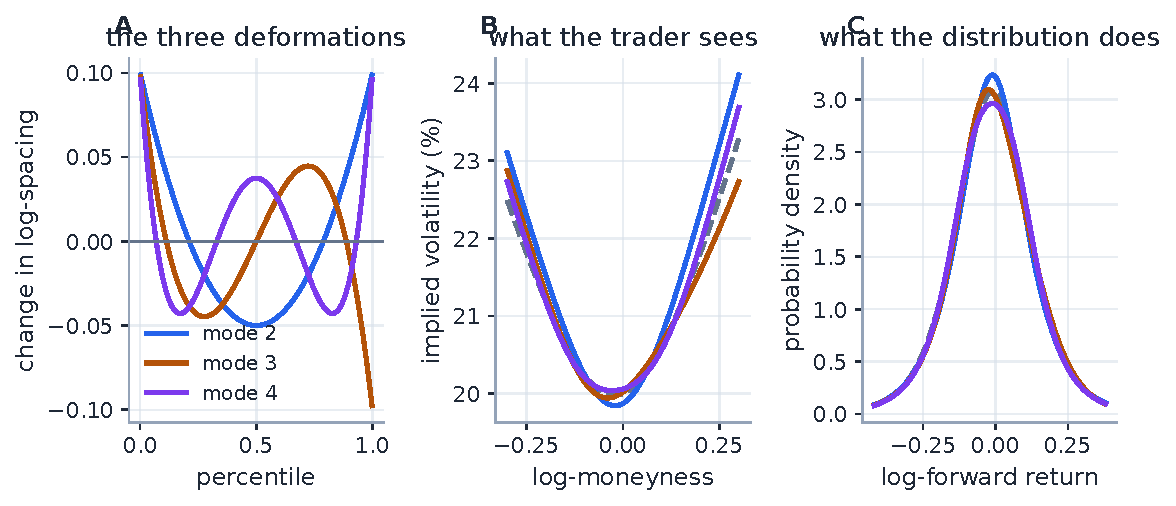
\includegraphics[width=\textwidth]{fig_lqd_fresh_modes.pdf}
\caption{One production basis coefficient at a time: $a_2$, $a_3$ or $a_4$
set to $0.10$ on the symmetric logistic reference of \cref{sec:logistic},
everything else untouched.  Panel A: the perturbation of $g$ --- a pure
Legendre mode in the rank, even ones symmetric, odd ones not.  Panel B: what
the trader sees --- mode 2 bends the smile symmetrically (butterfly), mode 3
tilts it (risk reversal), mode 4 works the shoulders.  Panel C: what the
distribution does --- mass leaves the stretched ranks and lands on the
compressed ones, and every deformed density is non-negative without anyone
checking.  The moral: \emph{body modes shuffle mass; endpoint terms own the
tails}.}
\label{fig:modes}
\end{figure}

%======================================================================
\section{An exactly solvable slice}
\label{sec:logistic}

Every lecture needs its harmonic oscillator.  Set all body modes to zero and
the two endpoint coefficients equal:
\begin{equation}
a_n=0,\qquad L=R=\log s
\qquad\Longrightarrow\qquad
g\equiv\log s,
\quad \frac{\dd Q}{\dd z}=s .
\end{equation}
The quantile is exactly linear in log-odds, $Q(z)=\mu+s\,z$; that is, $X$ is
a \emph{logistic} random variable with scale $s$:
$X=\mu+sZ$ with $Z=\log\frac{U}{1-U}$ for a uniform rank $U$.

Everything about this slice flows from one integral.  The moment generating
function of $Z$ is a rank integral we can actually do --- substituting
$e^{tZ}=\big(\tfrac{u}{1-u}\big)^{t}$ turns it into Euler's beta integral:
\begin{equation}
\E\big[e^{tZ}\big]
=\int_0^1\Big(\frac{u}{1-u}\Big)^{t}\dd u
=\mathrm{B}(1+t,\,1-t)
=\Gamma(1+t)\,\Gamma(1-t)
=\frac{\pi t}{\sin(\pi t)},
\qquad |t|<1 .
\label{eq:logistic_mgf}
\end{equation}
Note, in passing, that the formula itself confirms \cref{sec:tails}: it
exists exactly on the strip $|t|<1$, as it must for a law with $A_L=A_R=1$
per unit scale.  Two facts fall out of \eqref{eq:logistic_mgf} at once:
\begin{itemize}[leftmargin=1.4em]
\item \textbf{The martingale shift, exactly.}  Read it at $t=s$:
$\E[e^{sZ}]=\pi s/\sin(\pi s)$, so the shift that makes $e^{X}$ mean-one is
$\mu=-\log\big(\pi s/\sin(\pi s)\big)$ in closed form --- the only slice in
the family whose $\mu$ needs no quadrature.
\item \textbf{The variance, and hence the initializer.}  Expand its
logarithm at $t=0$: since $\sin(\pi t)=\pi t\,(1-\pi^{2}t^{2}/6+\cdots)$,
\[
\log\E\big[e^{tZ}\big]=\frac{\pi^{2}t^{2}}{6}+O(t^{4})
\qquad\Longrightarrow\qquad
\Var(Z)=2\cdot\frac{\pi^{2}}{6}=\frac{\pi^{2}}{3},
\]
the second cumulant being twice the quadratic coefficient.  So
$\Var(X)=\pi^{2}s^{2}/3$, and matching a target ATM total variance $w_0$
gives the seed $s\approx\sqrt{3w_0}/\pi$.
\end{itemize}
The remaining diagnostics are immediate: $A_L=A_R=s$, so the slice is
admissible iff $s<1$ (a 55\% vol at one year is $s\approx0.30$, nowhere near
the wall), and the Lee slopes are $\beta_L=\psi(1/s)$ and
$\beta_R=\psi(1/s-1)$ --- slightly asymmetric wings even for this symmetric
law, because the martingale shift tilts the smile.

This two-line model is precisely the production cold-start initializer ---
the \texttt{logistic\_init} routine of \texttt{models/lqd/calibrate.py}:
match $s$ to the ATM-interpolated quote variance, then let the optimizer
bend $L\ne R$ (tail asymmetry) and the $a_n$ (body).

\Cref{fig:ruler} walks the whole pipeline on a solved instance ---
production root-solving the scale so that the ATM volatility is
\emph{exactly} $20\%$ at $\tau=\lqdfreshtoyexpiry$ --- and it repays reading
one panel at a time.  Panel A is the coordinate itself: the log-odds line
holds every percentile of an unbounded law at finite coordinates, with equal
steps in $z$ meaning equal \emph{multiplications} of the odds (the 1st and
99th percentiles sit at $z=\mp4.6$, not at infinity).  Panel B is the law:
in rank coordinates the straight line $Q=\mu+sz$ becomes the gentle S-curve
shown, and one detail deserves a pause --- the forward ($k=0$, marked) sits
at the $\lqdfreshtoyuatmpct\%$ rank, \emph{above} the median.  That is the
martingale shift at work: for $e^{X}$ to average to one, the convexity of
the exponential demands a median return slightly below zero
($Q(\tfrac12)=\mu=\lqdfreshtoymu$), so more than half the outcomes finish
below the forward.  Jensen's inequality, drawn.  Panel C is the market's
view of the same object: a symmetric, gently convex smile pinned at
$20.00\%$ --- convex because exponential tails are heavier than the
log-normal's, so far strikes carry more relative value, which the Black
formula can only express as higher implied volatility.  The example box then
prices one option on this slice by hand.

\begin{figure}[H]
\centering
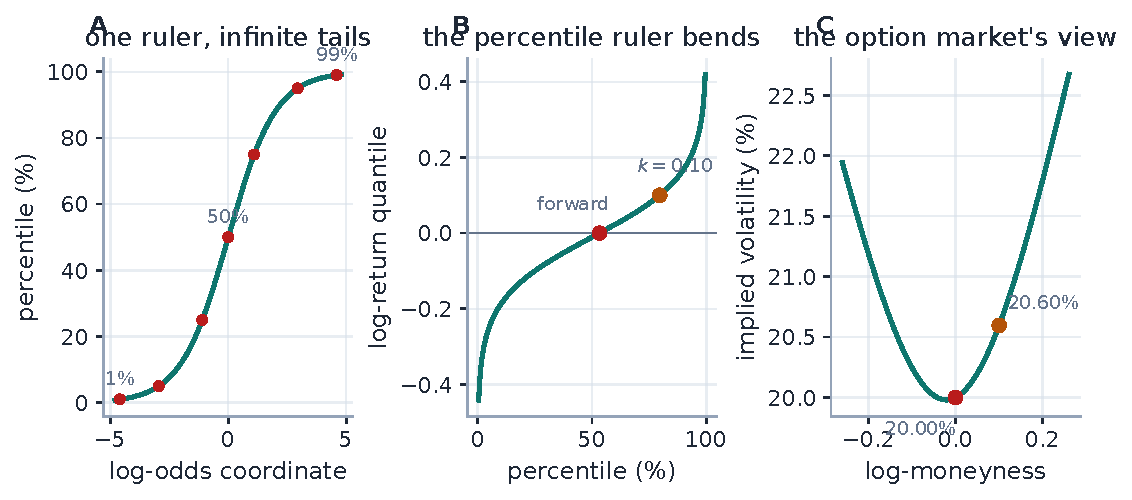
\includegraphics[width=\textwidth]{fig_lqd_fresh_ruler.pdf}
\caption{The exactly solvable slice, solved to an ATM volatility of exactly
20\% at $\tau=\lqdfreshtoyexpiry$ (production root-solve:
$s=\lqdfreshtoyscale$).  A: the log-odds ruler --- every percentile at a
finite coordinate.  B: the quantile in rank coordinates; the forward's rank
is $\lqdfreshtoyuatmpct\%>50\%$ because the martingale shift pushes the
median return down to $\mu=\lqdfreshtoymu$ (Jensen's inequality, drawn).
C: the resulting smile --- $20.00\%$ at the money by construction, convex
because exponential tails out-fatten the log-normal.}
\label{fig:ruler}
\end{figure}

\begin{example}[title={A trade ticket priced by hand}]
On the solved slice of \cref{fig:ruler}, price the $k=0.10$ call
($\approx10.5\%$ out of the money).  The strike's rank is
$u_{k}=\lqdfreshtoyuten$: the option finishes in the money with probability
$1-u_k\approx20.3\%$.  The two ledgers of \cref{sec:pricing} read
$G(z_k)=\lqdfreshtoyshareten$ (the share of the mean carried by outcomes
above the strike) and $e^{k}(1-u_k)=\lqdfreshtoycashten$ (the strike paid on
that event), so
\[
C(0.10)=G-\,e^{k}(1-u_k)=\lqdfreshtoycallten
\qquad\Longrightarrow\qquad
\sigma_{\text{imp}}=\lqdfreshtoyivten\%,
\]
about $0.6$ vol points above the ATM level: the first taste of a smile.
Production reproduces every number in this box to the displayed digits
(\texttt{gen\_lqd\_fresh.py}); the martingale check on the slice returns
$\E[e^{X}]-1=0$ to machine precision.
\end{example}

%======================================================================
\section{From coefficients to prices: one cumulative integral}
\label{sec:pricing}

The whole pricing pipeline is the arrow chain
\[
\theta\;\longrightarrow\;g\;\longrightarrow\;Q\;\longrightarrow\;\mu
\;\longrightarrow\;C(k)\;\longrightarrow\;\sigma(k),
\]
and this section makes each arrow one integral (or one root-solve) on a
single shared grid.

\subsection{The log-odds machine}

The skeleton's endpoint singularities are a feature for tails and a nuisance
for quadrature --- so we integrate in the coordinate that removes them.
Under $z=\log\frac{u}{1-u}$, by \eqref{eq:q_logit}, the quantile is the
integral of a smooth positive function on the whole line:
\begin{equation}
Q(z)=\mu+\int_0^{z}e^{g(u(s))}\,\dd s ,
\label{eq:Q_of_z}
\end{equation}
anchored at the median node $z=0$.  The shift is fixed by the martingale
condition, which in the same coordinate reads (using $\dd u = u(1-u)\,\dd z$)
\begin{equation}
\mu=-\log\!\left(
\int_{-\infty}^{\infty}
e^{\,Q(z)-\mu}\;u(z)\big(1-u(z)\big)\,\dd z\right),
\label{eq:mu_norm}
\end{equation}
one logarithm of one integral.  This is the \emph{only} normalization in the
model; being an additive shift of $Q$ it changes neither $q$, nor the tails,
nor positivity --- it slides the whole law along the return axis until the
forward is its mean.

Pricing needs one more cumulative object.  Define the \emph{upper share}
\begin{equation}
G(z)=\int_{z}^{\infty}e^{\,Q(s)}\,u(s)\big(1-u(s)\big)\,\dd s
\;=\;\E\big[\,Y\,\1_{\{Y>e^{Q(z)}\}}\big]:
\label{eq:upper_share}
\end{equation}
the share of the (unit) mean carried by outcomes above the rank $u(z)$.  It
falls from $G(-\infty)=1$ to $G(+\infty)=0$, and it prices every call at
once: if $z_k$ solves $Q(z_k)=k$, then, splitting the call payoff into asset
and cash legs,
\begin{equation}
C(k)=G(z_k)-e^{k}\,\big(1-u(z_k)\big).
\label{eq:call_price}
\end{equation}
The put is $P(k)=e^{k}u(z_k)-(1-G(z_k))$, and parity is immediate.  Equation
\eqref{eq:call_price} is worth staring at: an option price is the difference
of two ledgers, both monotone, both already on the grid.  The same $G$ will
hand us the analytic Jacobian in \cref{sec:jacobian} and the calendar
ordering in \cref{sec:calendar} --- one object, three jobs.

\subsection{What one build of a slice actually is}
\label{sec:quadrature}

It is worth being concrete here, because the entire calibrator stands on
this one loop being cheap and smooth.  Given a trial $\theta$, production
does five things, in order, on a fixed symmetric grid $z_j\in[-Z,Z]$:
\begin{enumerate}[leftmargin=1.6em]
\item evaluate $g$ at the (cached) ranks $u_j$ --- one matrix-vector
product, since $g$ is linear in $\theta$;
\item integrate $e^{g}$ cumulatively (fourth-order Simpson) to get the
unshifted quantile, anchored at the median node $z=0$;
\item compute the martingale integral, take one logarithm, and shift:
$Q\mathrel{+}=\mu$;
\item integrate $e^{Q}u(1-u)$ cumulatively \emph{from the right} to get the
upper share $G$;
\item stop.  Every strike, at any later moment, is priced from
\eqref{eq:call_price} by interpolating these two curves and solving one
root.
\end{enumerate}
Nothing here is iterative, nothing can fail for an admissible $\theta$, and
the cost is a few dense passes over one array.

Two details of this recipe deserve their ``why''.  The first is the
truncation at $|z|=Z$ (production: $Z=40$).  Beyond the grid the integrands
of steps 3 and 4 are, by \cref{sec:tails}, essentially exact exponentials
--- so instead of praying the tail is negligible, production \emph{sums it
in closed form}, appending the geometric-series corrections
\begin{equation}
\int_{Z}^{\infty}e^{Q}u(1-u)\,\dd z\approx\frac{e^{\,Q(Z)-Z}}{1-A_R},
\qquad
\int_{-\infty}^{-Z}e^{Q}u(1-u)\,\dd z\approx\frac{e^{\,Q(-Z)-Z}}{1+A_L}.
\label{eq:tail_corr}
\end{equation}
(Notice the right-hand denominator displaying the $A_R=1$ wall once more.)
For equity tail scales the corrections themselves are far below
double-precision noise at $Z=40$; they are kept because they make the build
exact-in-the-limit rather than merely truncated.

The second detail is how the two curves are read \emph{between} nodes.  The
construction hands us the exact nodal derivatives for free ---
$\dd Q/\dd z=e^{g}$ from \eqref{eq:q_logit} and $\dd G/\dd z=-e^{Q}u(1-u)$
from \eqref{eq:upper_share} --- and it would be wasteful not to use them:
production stores both and interpolates off-grid with \emph{cubic Hermite}
polynomials rather than linearly.  The payoff is threefold: priced curves
are smooth enough for clean finite-difference Greeks; the strike root
$Q(z_k)=k$ can be polished by Newton on the interpolant to machine
precision (which is what will make the ATM handles of \cref{sec:handles}
\emph{exact} rather than grid-limited); and because Hermite interpolation
returns the nodal value exactly at a node, a constraint expressed at grid
$z$-values --- the calendar floor of \cref{sec:calendar} --- matches its
node-indexed form bit for bit, whatever grid the optimizer runs on.

\begin{perfbox}
The grid $(z_j,u_j,u_j(1-u_j))$ and the Legendre matrix $P_n(1-2u_j)$ depend
only on $(Z,n_{\text{pts}},N)$ --- never on $\theta$.  A calibration builds
the slice many hundreds of times, so these arrays are LRU-cached and returned
read-only; only the parameter combination $g$ is re-formed per call, which
alone made \texttt{build\_slice} about $1.7\times$ faster.  Optimization
iterates on a coarser grid of \lqdoptpts\ nodes (Simpson error already orders
of magnitude below the fit budget) and the accepted slice is rebuilt once at
the full $8001$ nodes for reporting, density, var-swap and calendar
diagnostics.  Converged parameters agree with a full-grid fit to
$\sim10^{-6}$.  See \cref{app:perf}.
\end{perfbox}

\subsection{Back to the quoted smile}
\label{sec:black}

The market speaks implied volatility, so the last arrow inverts Black.  In
normalized total-variance units,
\begin{equation}
\Black(k,w)=\PhiN(d_+)-e^{k}\,\PhiN(d_-),
\qquad
d_\pm=-\frac{k}{\sqrt w}\pm\frac{\sqrt w}{2},
\label{eq:black}
\end{equation}
and the model's total implied variance solves $\Black(k,w(k))=C(k)$ ---
a scalar root per strike, monotone in $w$, safe for Newton.

Calibration, however, deliberately does \emph{not} fit in volatility space.
Given a quote $\sigma_i$ at $k_i$, with $w_i=\sigma_i^{2}\tau$, the residual
is the \emph{vega-normalized price error}
\begin{equation}
r_i(\theta)
=\frac{C(k_i;\theta)-\Black(k_i,w_i)}
{\partial_\sigma\Black(k_i,w_i)+\eta},
\qquad
\partial_\sigma\Black=\phin(d_+)\sqrt{\tau},
\label{eq:vega_resid}
\end{equation}
with a small floor $\eta$ against the vanishing far-wing vega
(\cref{app:atlas}).  Working in price space keeps every iterate a valid law
(no implied-vol inversion inside the loop, no inversion failures on wild
iterates); dividing by vega undoes the price-to-vol scale so the optimizer
still sees, to first order, a volatility error.  The error \emph{ledger} the
note reports --- always in vol basis points --- is computed after
convergence by honest Black inversion.

%======================================================================
\section{Three exact handles, and a chart built around them}
\label{sec:handles}

\subsection{Level, skew, curvature in closed form}
\label{sec:atm_exact}

Traders want the leading coordinates of a smile model to be the \emph{actual}
ATM volatility, skew and curvature --- not proxies, not finite differences
of a plotted curve.  The LQD slice delivers all three exactly, and the
derivation is three short steps: read two numbers off the law, pin the ATM
level, then push everything through the Black formula with the chain rule.
Recall the convention of \cref{tab:ledger}: primes are $k$-derivatives of
one-variable curves ($C$, $w$, $\sigma$), subscripted $\partial$'s are
partials of the two-variable $\Black(k,w)$; everything below is evaluated at
the money.

\paragraph{Step 1: two numbers from the law.}  Differentiate the rank-form
call $C(k)=\int_{u_k}^1(e^{Q(u)}-e^{k})\,\dd u$ in $k$.  The moving boundary
$u_k$ contributes nothing --- the integrand vanishes exactly there, an
envelope fact that returns in force in \cref{sec:jacobian} --- so only the
$-e^{k}$ inside survives: $C'(k)=-e^{k}(1-u_k)$.  Differentiating once more
brings in the density, since $\dd u_k/\dd k=f_X(k)$.  At $k=0$, writing
$u_0$ for the forward's rank ($Q(u_0)=0$) and
$f_0=u_0(1-u_0)e^{-g(u_0)}$ for the ATM density \eqref{eq:density},
\begin{equation}
C'(0)=-(1-u_0),
\qquad
C''(0)=f_0-(1-u_0).
\label{eq:Cder}
\end{equation}

\paragraph{Step 2: the ATM level.}  At $k=0$ the Black formula collapses,
and the ATM total variance $w_0$ is pinned by one monotone scalar equation,
\begin{equation}
\Black(0,w_0)=2\,\PhiN\!\Big(\frac{\sqrt{w_0}}{2}\Big)-1=C(0).
\label{eq:atm_level}
\end{equation}

\paragraph{Step 3: the chain rule through Black.}  The model's smile is
\emph{defined} by the identity $\Black\big(k,w(k)\big)=C(k)$.
Differentiating it once and twice at $k=0$,
\[
\partial_k\Black+\partial_w\Black\,w'=C',
\qquad
\partial_{kk}\Black+2\,\partial_{kw}\Black\,w'
+\partial_{ww}\Black\,(w')^{2}+\partial_w\Black\,w''=C'',
\]
and solving for the two unknowns,
\begin{equation}
w'(0)=\frac{C'(0)-\partial_k\Black}{\partial_w\Black},
\qquad
w''(0)=\frac{C''(0)-\partial_{kk}\Black
-2\,\partial_{kw}\Black\;w'(0)-\partial_{ww}\Black\;w'(0)^{2}}
{\partial_w\Black}.
\label{eq:w_derivs}
\end{equation}
The five ATM Black partials are classical; with the shorthands
$a=\sqrt{w_0}/2$, $\PhiN_a=\PhiN(a)$, $\phin_a=\phin(a)$,
\begin{equation}
\begin{aligned}
\partial_k\Black&=-(1-\PhiN_a), &
\partial_w\Black&=\tfrac{\phin_a}{2\sqrt{w_0}}, &
\partial_{kk}\Black&=-(1-\PhiN_a)+\tfrac{\phin_a}{\sqrt{w_0}},\\
\partial_{kw}\Black&=\tfrac{\phin_a}{4\sqrt{w_0}}, &
\partial_{ww}\Black&=-\tfrac{\phin_a}{4w_0^{3/2}}-\tfrac{\phin_a}{16\sqrt{w_0}}. & &
\end{aligned}
\label{eq:black_partials}
\end{equation}
Finally, translate total variance into volatility: $\sigma(k)=\sqrt{w(k)/\tau}$,
so one more application of the same chain rule yields the handles,
\begin{equation}
\sigma_0=\sigma(0)=\sqrt{\frac{w_0}{\tau}},
\quad
s_0=\sigma'(0)=\frac{w'(0)}{2\sqrt{\tau w_0}},
\quad
\kappa_0=\sigma''(0)=\frac{w''(0)}{2\sqrt{\tau w_0}}
-\frac{w'(0)^{2}}{4\sqrt{\tau}\,w_0^{3/2}}.
\label{eq:atm_handles}
\end{equation}
Every quantity along the route is closed-form or one scalar root, so the
handles are exact for every LQD slice: the level in volatility units
(annualized on the active clock $\tau$), the skew in vol per unit
log-moneyness, the curvature in vol per unit log-moneyness squared.

\begin{remark}[One triple, two unit systems]
Production carries this information in two \emph{equivalent} coordinate
systems: the graph-facing carrier $(\sigma_0,s_0,\kappa_0)$ that Note~14
propagates, and the internal chart's $H=(w_0,s_0,\kappa_0)$ with the ATM
total variance first (\texttt{models/lqd/ortho.py}).  Since
$w_0=\sigma_0^{2}\tau$, the two are a smooth bijection --- no information is
at stake, only the \emph{units} of the first coordinate.  The reason to be
pedantic is that a volatility handed where a total variance is expected
fails silently; so the note fixes the convention once --- $H$ always means
the total-variance triple --- and the graph adapter converts.
\end{remark}

\begin{heuristic}
Equation \eqref{eq:Cder} is the distribution speaking directly.  $-C'(0)$ is
the probability of finishing above the forward --- the ATM digital --- and
the skew in \eqref{eq:w_derivs} is, at heart, the mismatch between that
digital and the $\PhiN(d_-)$ the Black model would assign it.  The curvature
adds one more distributional fact, the ATM density $f_0$.  Level, digital,
density: three numbers of the law, three handles of the smile.
\end{heuristic}

\subsection{The ATM-orthogonal chart}
\label{sec:ortho}

The handles earn their keep when they stop being diagnostics and become
\emph{coordinates}: axes of parameter space that a person can hold.  What we
want is a chart around the current fit whose first three axes \emph{are}
level, skew and curvature, and whose remaining axes deliberately do nothing
to them.  Building it amounts to answering two questions, and each answer is
a subspace.

Fix the reference $\theta^{*}$ (in practice, the freshly fitted slice),
write $H(\theta)=(w_0,s_0,\kappa_0)\in\R^{3}$ for the handle map, and let
$J=\partial H/\partial\theta\in\R^{3\times d}$ be its Jacobian at
$\theta^{*}$ --- computed by central differences, which on this
deterministic, smooth quadrature is accurate to $\sim10^{-9}$.

\emph{Question 1: what is the cheapest way to move the handles?}  A
perturbation $\delta\theta$ moves them by $J\,\delta\theta$ to first order,
so a prescribed handle move $\delta H$ means three equations in $d$
unknowns --- underdetermined, many solutions.  Take the shortest one:
\begin{equation}
\delta\theta=U\,\delta H,
\qquad
U=J\T(JJ\T)^{-1},
\label{eq:primary_dirs}
\end{equation}
the least-norm right inverse of $J$, so that $JU=I_3$.  The three columns
of $U$ are the \emph{primary directions}: moving along them changes the
handles one-for-one, in handle units, with no wasted motion in parameter
space.

\emph{Question 2: which moves leave the handles alone?}  To first order,
exactly the kernel of $J$ --- a $(d-3)$-dimensional space.  Collect an
orthonormal basis of it as the columns of $V$; these are the \emph{shape
directions}.

Gluing the two answers together gives the chart:
\begin{equation}
\theta=\theta^{*}+U\alpha+V\xi,
\label{eq:ortho_chart}
\end{equation}
with three coordinates $\alpha$ that read directly as handle moves ---
$H\approx H(\theta^{*})+\alpha$ --- and $d-3$ coordinates $\xi$ that
reshape wings, shoulders and event convexity while the handles stand
still.

First order is not forever, so production closes the gap.  To hit a target
$H^{\text{target}}$ \emph{exactly}, it solves the three-dimensional system
$H(\theta^{*}+U\alpha+V\xi)=H^{\text{target}}$ for $\alpha$ by Newton ---
and here the construction pays for itself twice, because $JU=I_3$ makes the
system's Jacobian the identity at the reference: the natural first guess
$\alpha=H^{\text{target}}-H(\theta^{*})$ is already excellent, and the
preconditioner rarely needs refreshing.  This \emph{retarget} is what lets a
trader drag ATM level, skew or curvature while the optimizer keeps the
shape modes for everything else; \cref{fig:ortho} shows one move of each
kind on the running example.

\begin{figure}[H]
\centering
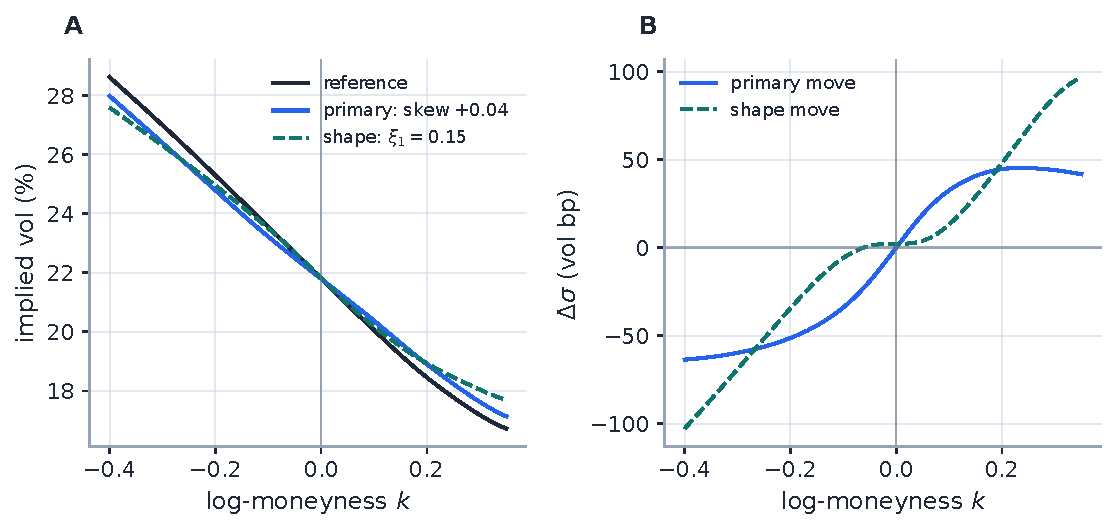
\includegraphics[width=\textwidth]{fig_lqd_geom_ortho.pdf}
\caption{The chart in action on the running SPX-like fit ($d=10$, so
$\lqdgeomnshape$ shape directions).  Panel A: the reference smile; a
\emph{primary} move retargeting the skew by $+\lqdgeomskewbump$ exactly
(achieved to $\lqdgeomretargetresid$ by the Newton solve) with level and
curvature held; and a \emph{shape} move along the first kernel direction.
Panel B: the same two moves as differences.  The primary move tilts the smile
through the money; the shape move relocates over $\lqdgeomshapewingmove$
vol bp of wing while drifting the ATM level by only
$\lqdgeomshapedriftsigma$ vol bp, the skew by $\lqdgeomshapedriftskew$ and
the curvature by $\lqdgeomshapedriftcurv$ --- first-order invariance visible
to the eye as a flat spot at the money.}
\label{fig:ortho}
\end{figure}

\begin{caution}
The chart is \emph{local}: $U$ and $V$ are frozen at $\theta^{*}$, so the
handle-invariance of shape directions degrades quadratically with the
excursion (the residual drift in \cref{fig:ortho} is exactly that second
order), and the retarget Newton solve can fail --- or converge to an
\emph{infeasible} point --- when the requested handles push the slice toward
the $A_R=1$ wall (a large curvature demand on a thin-tailed reference is the
classic case).  Callers must treat retargeting as an operation that can
fail near the wall, not as a total map on handle space.
\end{caution}

%======================================================================
\section{Calibrating one expiry}
\label{sec:calib}

We have spent eight sections building a space in which every point is an
arbitrage-free slice.  Choosing the \emph{right} point is now almost an
anticlimax --- which was the design goal all along.  This section states the
objective, the one place it must brake (the wall), where fits start from,
and how the shipped objective is actually assembled.

\subsection{The core objective}

Given quotes $(k_i,\sigma_i)$ at one expiry, the calibrator solves the
bound-free nonlinear least-squares problem (scipy \texttt{trf})
\begin{equation}
\min_{\theta}\;
\sum_i r_i(\theta)^{2}
\;+\;\lambda\sum_{n\ge4}n^{2r}a_n^{2},
\label{eq:calib_objective}
\end{equation}
with $r_i$ the vega-normalized residuals \eqref{eq:vega_resid}.  (An
optional per-quote weighting --- Note~07's \texttt{weightScheme} ---
multiplies the residuals; it changes nothing below and we suppress it.)
The high-order ridge $\lambda\,n^{2r}a_n^{2}$ is optional; it suppresses
oscillation in sparse markets while deliberately leaving the first body modes
$a_2,a_3$ --- the workhorses of curvature and asymmetry --- untouched.  Note
what is \emph{absent}: there is no density-positivity term anywhere, because
positivity is structural (\cref{prop:nobutterfly}).  The one admissibility
condition is the wall \eqref{eq:AR_wall}, enforced as
$A_R<1-\eps_R$ with a tiny buffer, plus the smooth barrier below.

\subsection{The soft turn before the hard wall}

To keep the residual smooth as the optimizer approaches $A_R=1$, the stacked
residual carries a softplus barrier row
\begin{equation}
b(\theta)=\log\!\big(1+e^{\,\gamma\,(A_R-c)}\big),
\label{eq:barrier}
\end{equation}
with centre $c=\lqdbarriercenter$ and steepness $\gamma=\lqdbarrierscale$
(both \texttt{FitSettings} coefficients; evaluated as
$\operatorname{logaddexp}(0,\cdot)$, so a wild trial $\theta$ cannot overflow
it).  The barrier is negligible for $A_R\ll c$ and rises steeply near the
wall, turning the fit around \emph{before} the hard rejection; if a trial
$\theta$ does cross $A_R\ge1$, the price block is replaced by a large
penalty increasing smoothly in $A_R$, so the trust region still sees a
gradient pointing back to feasibility.

\subsection{Initialization and warm starts}

The only cold-start initializer in production is the exactly solvable slice
of \cref{sec:logistic}: $a_n=0$, $L=R=\log s$ with $s=\sqrt{3w_0}/\pi$ from
the variance match, seeded from the ATM-interpolated quote variance.
Sequential workflows do better than cold: the background Calibrate sweep
\emph{warm-starts} each expiry from the previous, shorter-dated expiry's
freshly fitted parameters (adjacent maturities have nearly the same smile, so
\texttt{trf} lands close to the optimum), and the service can also run a
\emph{data-only prepass} --- a persistence-free fit used as the measurement
stage of the prior and filter machinery (Notes~13 and 15).  Wing-aware and
quantile-projection initializers are roadmap items, not shipped code.

\subsection{The full residual stack}
\label{sec:stack}

The two-term objective \eqref{eq:calib_objective} is the lecture version.
The shipped objective is a \emph{stack} of residual blocks, and
\cref{tab:stack} is the map of the whole territory: the data block and ridge
we have met, the calendar slack of \cref{sec:calendar}, the barrier, and
then a run of optional blocks --- var-swap targets, priors, filter terms ---
each of which belongs to its own note in the series and simply plugs extra
rows into the same least-squares problem.  Two properties of the assembly
are worth carrying away.  Every optional block is byte-identical-to-absent
when unused (test-locked), so switching a feature off really is off.  And
the Jacobian column matters operationally: the analytic route of
\cref{sec:jacobian} covers the first five blocks, while activating \emph{any}
var-swap or prior block switches the whole fit to scipy's finite-difference
Jacobian --- correct, merely not accelerated.

\begin{table}[H]
\centering\small
\setlength{\tabcolsep}{4pt}
\begin{tabular}{@{}p{0.24\textwidth}p{0.26\textwidth}p{0.24\textwidth}l@{}}
\toprule
Residual block & Active when & Units / scaling & Jacobian\\
\midrule
Mid data block & \texttt{fitMode=mid} (default) & vega-normalized price
($\approx$ vol) & analytic\\
Band data block (hinge $+$ mid anchor; Note~07) & \texttt{fitMode}
\texttt{bidask}/\texttt{haircut} & vega-normalized price & analytic\\
High-order ridge & \texttt{regLambda}$>0$ (rows $n\ge4$) & coefficient units &
analytic\\
Calendar slack (Note~10) & \texttt{enforceCalendar} $+$ a nearer fitted expiry
& upper share (normalized price) & analytic\\
$A_R$ soft barrier & always (one row) & dimensionless & analytic\\
\midrule
Market var-swap (Note~08) & \texttt{varSwapEnabled} $+$ an active quote &
vol & FD fallback\\
Prior strike-gap anchor (Note~13) & \texttt{strike\_gap} / \texttt{hybrid}
tail, active prior & vega-normalized price & FD fallback\\
Prior var-swap companion (Note~13) & alongside an active prior & vol & FD
fallback\\
Operator prior (Note~13) & \texttt{quote\_operator} / \texttt{hybrid}, gated
per operator & operator units (vol) & FD fallback\\
Active-filter MAP (Note~15) & filter mode \texttt{active} (rides the operator
block, ungated) & handle units & FD fallback\\
\bottomrule
\end{tabular}
\caption{The LQD residual stack as production assembles it
(\texttt{models/lqd/calibrate.py}; prior/filter targets are resolved in
\texttt{api/service.py}).  ``FD fallback'' means the presence of that block
switches the entire fit to the finite-difference Jacobian.}
\label{tab:stack}
\end{table}

\subsection{The native var-swap route}
\label{sec:varswap}

The log-contract identity gives the var-swap proxy in one line of the
model's own coordinates:
\begin{equation}
w_{\text{vs}}=-2\,\E[X]
=-2\int_{-\infty}^{\infty}Q(z)\,u(z)\big(1-u(z)\big)\,\dd z,
\label{eq:varswap}
\end{equation}
a single quadrature on the grid the slice already owns, with integrand
decaying like $z\,e^{-|z|}$ (\texttt{quadrature.py::var\_swap\_strike}).  Two
qualifications keep the claim honest.  First, this native route is
dramatically cheaper than the generic strike replication of Note~08 --- which
would re-solve implied variance on a strike grid at every Jacobian column
--- but activating the var-swap block also forfeits the analytic Jacobian
(\cref{tab:stack}), so a var-swap fit is not literally as cheap as a mid fit.
Second, the identity prices the \emph{log contract}: its correspondence with
a realized-variance swap assumes continuous monitoring of a continuous
(diffusive) path; jumps and discrete sampling take the usual corrections,
outside this model's scope.

%======================================================================
\section{The derivative that comes free}
\label{sec:jacobian}

The dominant cost of \eqref{eq:calib_objective} used to be the Jacobian:
scipy rebuilt the entire quadrature pipeline $P+1$ times per iteration to
finite-difference it, with $P=N+1$ the parameter count.  The Vol-Fitter
instead propagates the analytic Jacobian of the core residual stack --- data
block (mid or band), ridge, calendar slack, barrier --- in \emph{one}
quadrature pass.  The key is a cancellation identity, and it is the cleanest
piece of mathematics in the implementation.

\subsection{The cancellation identity}

The subtlety is that the priced call \eqref{eq:call_price} depends on
$\theta$ twice: explicitly through the curves $Q$ and $G$, and implicitly
through the strike root $z_k(\theta)$ solving $Q(z_k;\theta)=k$.  A naive
gradient must differentiate the root.  Differentiate the pricing identity
and watch:
\begin{equation}
\frac{\dd C}{\dd\theta}
=\underbrace{\frac{\partial G}{\partial\theta}\Big|_{z=z_k}}_{\text{explicit}}
+\Big[\,G'(z_k)+e^{k}\,u'(z_k)\Big]\frac{\dd z_k}{\dd\theta} .
\end{equation}
Now $G'(z)=-e^{Q(z)}u(1-u)$ from \eqref{eq:upper_share}, while at the root
$e^{Q(z_k)}=e^{k}$ and $u'(z_k)=u_k(1-u_k)$.  The bracket is
\begin{equation}
-e^{k}u_k(1-u_k)+e^{k}u_k(1-u_k)=0 .
\end{equation}

\begin{theorem}[Implicit-root cancellation]
\label{thm:cancel}
The implicit dependence of the strike root on the parameters drops out of the
price gradient:
\begin{equation}
\frac{\dd C}{\dd\theta}
=\left.\frac{\partial G}{\partial\theta}\right|_{z=z_k}.
\label{eq:dC}
\end{equation}
\end{theorem}

\begin{remark}
This is an envelope argument in disguise.  $C(k)$ is an integral whose lower
limit $z_k$ sits exactly where the integrand of the combined asset-and-cash
ledger vanishes --- the payoff $(e^{Q}-e^{k})$ is zero at its own exercise
boundary --- so moving the boundary is free, to first order.  The same
mechanism makes the American exercise boundary drop out of American option
Greeks.
\end{remark}

So $\dd C/\dd\theta$ is obtained by evaluating the \emph{nodal} parameter
sensitivities of the upper share at the fixed point $z_k$ --- by the very
Hermite interpolation used to price, fed
$\partial G/\partial\theta_j$ and $\partial G'/\partial\theta_j$ instead of
the nodal values.

\subsection{Nodal sensitivities in one pass}

With the root out of the way, there is nothing left to invent: we simply
differentiate the five-step recipe of \cref{sec:quadrature}, step by step,
and every step stays a cumulative integral.  Two structural facts make it
painless.  First, $g$ is \emph{affine} in $\theta$, with constant basis
$\phi_j=\partial g/\partial\theta_j$ --- namely $\phi_L=1-u$, $\phi_R=u$,
$\phi_{a_n}=P_n(1-2u)$ --- so differentiating anything of the form $e^{g}$
just multiplies it by a fixed, cached array.  Second, integration and
$\partial/\partial\theta_j$ commute, so a derivative of a cumulative
integral is the cumulative integral of the derivative.

Walk the recipe.  Step 2 (the unshifted quantile $\overline Q=Q-\mu$)
differentiates under the integral sign,
\begin{equation}
\frac{\partial\overline Q(z)}{\partial\theta_j}
=\int_0^{z}e^{g}\,\phi_j\,\dd s ,
\end{equation}
one more cumulative Simpson pass per parameter.  Step 3 (the shift
$\mu=-\log M$, with $M$ the martingale integral) is a logarithm, so
\begin{equation}
\frac{\partial\mu}{\partial\theta_j}
=-\frac{1}{M}\int e^{\overline Q}\,
\frac{\partial\overline Q}{\partial\theta_j}\,u(1-u)\,\dd z
\;+\;(\text{tail-correction terms}),
\end{equation}
where the corrections \eqref{eq:tail_corr} contribute through
$\overline Q(\pm Z)$ and through $A_L,A_R$ --- whose own gradients cost
nothing, since \eqref{eq:endpoint_scales} gives
$\partial A_L/\partial\theta=A_L\,(1,0,1,1,\dots)$ and
$\partial A_R/\partial\theta=A_R\,(0,1,1,-1,\dots)$ with signs $(-1)^{n}$.
Step 4 (the share) is another cumulative pass: with
$\partial Q=\partial\mu+\partial\overline Q$ in hand, integrate
$\partial(e^{Q}u(1-u))/\partial\theta_j$ from the right, add its right-tail
correction, and note that the nodal slope sensitivity
$\partial G'/\partial\theta_j$ is the same integrand negated --- exactly
the pair the Hermite interpolant wants.  The non-price rows of the stack
then differentiate in one line each: the band hinge multiplies
$\dd C/\dd\theta$ by the violation sign, the ridge is diagonal on the
$a$-columns, the calendar slack reuses the share sensitivity at the
constraint nodes, and the barrier row is
$\expit\!\big(\gamma(A_R-c)\big)\,\gamma\,\partial A_R/\partial\theta$.
One quadrature pass, all $P$ columns.

One honesty note on exactness.  \Cref{thm:cancel} is exact for the
\emph{continuous} objects.  The discretization interpolates $Q$ and $G$ as
two separate Hermite interpolants, so between nodes the interpolated price is
not algebraically the integral of the interpolated quantile, and the
implemented gradient inherits that (tiny) mismatch.  The operational claim is
therefore \emph{benchmarked numerical agreement}, not algebraic identity ---
and it is benchmarked twice over, in \cref{fig:jacobian}.

\begin{figure}[H]
\centering
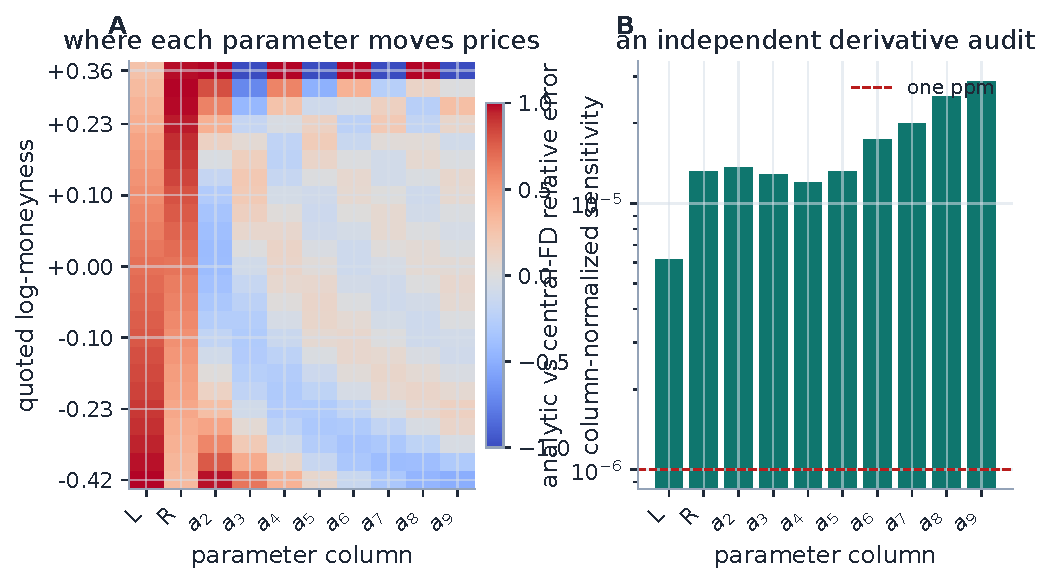
\includegraphics[width=\textwidth]{fig_lqd_fresh_jacobian.pdf}
\caption{The analytic Jacobian audited against an independent central finite
difference on the running fit ($\lqdfreshjacnparams$ parameters).  Panel A:
where each parameter moves prices --- $L$ and $R$ own the wings, each
Legendre mode paints its own oscillation across the strike ladder.  Panel B:
column-wise relative disagreement between the one-pass analytic Jacobian and
the central difference: at most $\lqdfreshjacmaxrel$, i.e.\ agreement to
about five significant digits of a derivative computed by a completely
different route.}
\label{fig:jacobian}
\end{figure}

\subsection{Scope and measured speed-up}

The analytic route covers the var-swap-free, prior-free configuration
(\cref{tab:stack}); other fits fall back to scipy's two-point finite
difference.  \Cref{tab:timing} and \cref{fig:timing} report a fresh
measurement: analytic and finite-difference fits reach the same optimum
(costs agreeing to $\sim10^{-11}$ relative, parameters to
$\lesssim10^{-5}$) with the analytic Jacobian $1.3$--$1.7\times$ faster
across $N=6\ldots12$.  Scope of the measurement: it times the least-squares
residual path on the synthetic benchmark, single-threaded, warm static-grid
cache, core residual blocks only --- different hardware, cache state, or an
active optional block moves the ratio.

\begin{table}[H]
\centering
\caption{Analytic vs.\ two-point finite-difference Jacobian, fresh run of the
production calibrator on the SVI-JW benchmark (fastest of three repeats,
single-threaded, warm cache, core residual blocks only).  $P=N+1$ is the
parameter count; the cost column confirms the same optimum within tolerance.}
\label{tab:timing}
\lqdtimingtable
\end{table}

\begin{figure}[H]
\centering
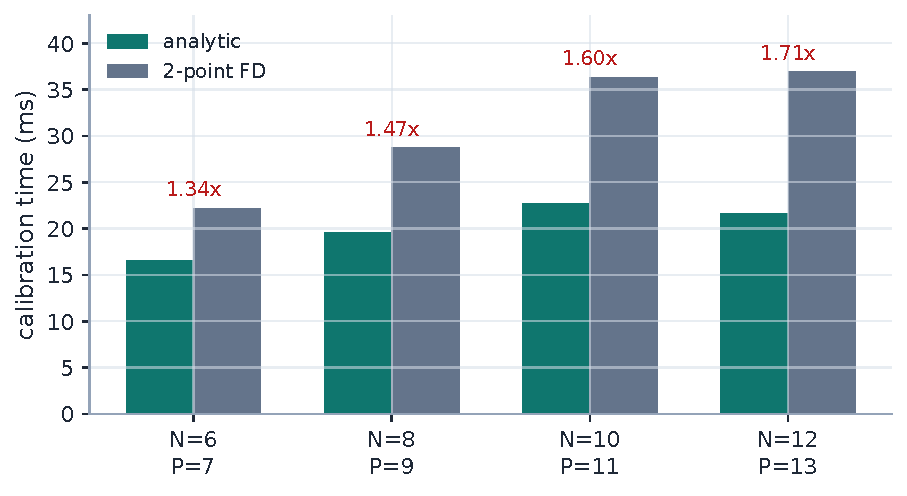
\includegraphics[width=0.78\textwidth]{fig_lqd_jacobian_timing.pdf}
\caption{The same measurement drawn: per-fit wall time with the analytic
one-pass Jacobian vs the $(P{+}1)$-rebuild finite difference, with the ratio
above each pair.  The win grows with the parameter count, as it must ---
the analytic pass costs one quadrature regardless of $P$.}
\label{fig:timing}
\end{figure}

\begin{heuristic}
Why only $\sim1.5\times$ and not $\sim P\times$?  Two reasons.  First, the
cached static grid makes a \emph{repeat} \texttt{build\_slice} cheap, so
$P+1$ finite-difference rebuilds cost much less than $P+1$ cold builds.
Second, \texttt{trf} converges here in a handful of iterations, so linear
algebra and the value evaluation dilute the Jacobian saving.  The structural
payoff --- a Jacobian that no longer rebuilds the quadrature --- is what
makes higher-order and surface-wide fits comfortable.
\end{heuristic}

%======================================================================
\section{Many expiries: order the ledgers}
\label{sec:calendar}

One dimension of the problem has been silent so far: time.
\Cref{prop:nobutterfly} silences butterflies \emph{within} a slice, but a
surface is many slices, and fitting them independently leaves a second
static arbitrage on the table: nothing yet prevents a longer-dated call from
pricing \emph{below} a shorter-dated one at the same log-moneyness --- a
calendar spread the market would pay you to own.  (Two standing assumptions
frame everything here: carry is deterministic, so normalized units under
each expiry's forward measure are legitimate simultaneously; and every slice
is normalized to mean one.)  For expiries $\tau_i<\tau_j$, absence of
calendar arbitrage is the requirement $C_i(k)\le C_j(k)$ at every $k$ ---
in the language of probability, the laws of $Y$ must increase in
\emph{convex order} \cite{Strassen1965}: the longer-dated law is more
spread out, worth at least as much against every convex payoff, without its
mean moving.

Checking a continuum of call inequalities sounds like work.  The pleasant
surprise is that the model already owns the right test object, because the
call curve and the upper share are \emph{Legendre transforms of each
other}.  For any rank $u$ and any log-strike $k$,
\begin{equation}
G(u)-e^{k}(1-u)
=\int_u^1\big(e^{Q(v)}-e^{k}\big)\,\dd v
\;\le\;C(k),
\end{equation}
because extending the integral to where the integrand is negative can only
lose money --- with equality exactly at $u=u_k$, the strike's own rank.
(That equality \emph{is} the pricing identity \eqref{eq:call_price},
rediscovered as a maximization.)  Read once in each direction:
\begin{equation}
C(k)=\max_{u\in[0,1]}\big[G(u)-e^{k}(1-u)\big],
\qquad
G(u)=\min_{k}\big[C(k)+e^{k}(1-u)\big].
\label{eq:legendre_dual}
\end{equation}
Each curve is an extremum over the other, and pointwise domination passes
through maxima and minima in both directions.  Hence, for mean-one slices,
\begin{equation}
C_i(k)\le C_j(k)\ \ \text{for all }k
\qquad\Longleftrightarrow\qquad
G_i(u)\le G_j(u)\ \ \text{for all }u\in[0,1],
\label{eq:calendar}
\end{equation}
with equality at $u=0$, where both shares equal the common mean, one.  A
continuum of option inequalities has become the pointwise ordering of two
curves that are already on the grid --- the same ledger that priced the
calls and carried the Jacobian, now doing its third job.

Enforcement follows the geometry.  The surface is built
nearest-to-farthest: each new slice is fitted subject to
$G_j(u_m)\ge G_i(u_m)$ on a dense rank grid (per-node slack tolerance zero
in production), as the soft calendar block of \cref{tab:stack} with penalty
weight \texttt{calendarWeight}; the constraint is evaluated at $z$-values,
so it is exact whatever grid the optimizer runs on
(\cref{sec:quadrature}).  Rank space is also the better-conditioned place to
test: no implied-volatility inversion at any strike, and full meaning
retained in the far wings, exactly where inversion goes blind.

\begin{figure}[H]
\centering
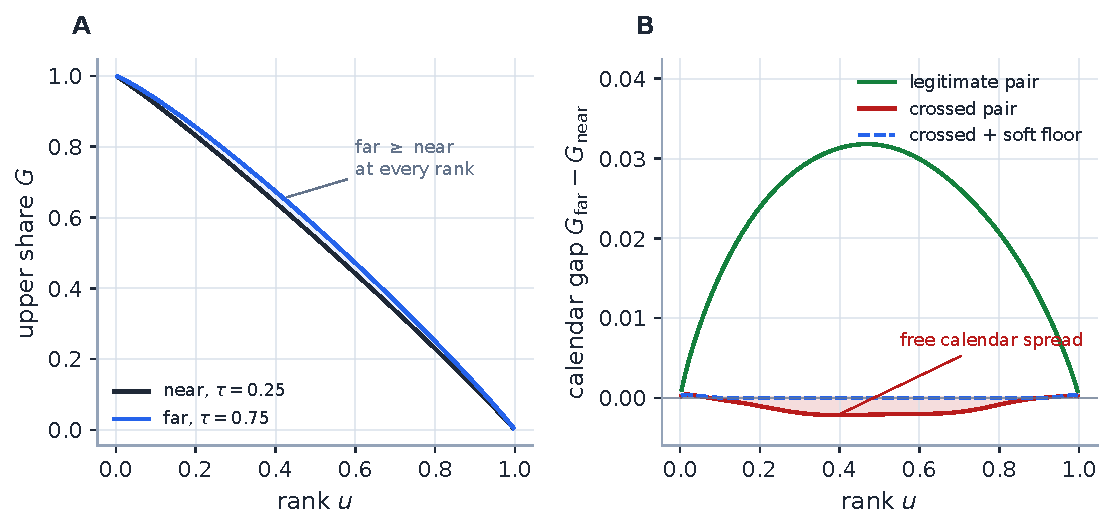
\includegraphics[width=\textwidth]{fig_lqd_geom_calendar.pdf}
\caption{Convex order on the ledger, three ways.  Panel A: upper shares of a
legitimate near/far pair (the running example and a proportionally scaled
quarter-year slice) --- both start at the common mean and the far curve
dominates.  Panel B: the calendar gap $G_{\text{far}}-G_{\text{near}}$.
Green: the legitimate pair stays non-negative (minimum
$\lqdgeommingaplegit$).  Red: a crafted far slice whose body variance sits
below the near slice dips to $\lqdgeommingapcross$ near the
$u\approx\lqdgeomugapcross$ rank --- calendar arbitrage a strike-space
inspection of two decent-looking smiles would not shout about.  Dashed blue:
the same crossed quotes refitted with the production soft floor; the
violation collapses to $\lqdgeommingaphealed$ --- pressed against zero from
below, visibly soft, visibly working.}
\label{fig:calendar}
\end{figure}

Honesty about the guarantee: this is \emph{control}, not a theorem.  The
hinge carries a finite weight, so a hard-pressed fit can retain a small
violation rather than destroy the quote fit (the dashed curve of
\cref{fig:calendar} retains exactly $\lqdgeommingaphealed$); the whole
coupling is a user toggle (\texttt{enforceCalendar}), and off means off;
residual violations are measured and reported by the surface diagnostics
rather than assumed away.  Note~10 develops the model-agnostic calendar
machinery (and the subtlety that the variance floor must be confined to the
traded strike range); here we record only that for LQD the natural constraint
object is the ledger the model already owns.

%======================================================================
\section{Case files}
\label{sec:cases}

A lecture should end with the machine run end-to-end, and with the operator
saying plainly what the run does and does not prove.  Both cases here come
from the generator \texttt{gen\_lqd\_fresh.py} in
\texttt{Docs/notes/figures} (the running example's numbers also feed
\texttt{gen\_lqd\_geometry.py}), fitting the production calibrator --- not
a notebook re-implementation --- against two deterministic targets.  What they prove is \emph{approximation capacity}:
that the basis can reproduce a known clean curve through option prices and
back.  What they do not prove is market fit; that evidence, against noisy
NBBO quotes, lives in the backtest reports (\cref{sec:problem}).
\Cref{tab:cases} puts the two side by side.

\begin{table}[H]
\centering
\caption{The two case files at a glance (fresh production run).}
\label{tab:cases}
\lqdfreshfitdiagtable
\end{table}

\subsection{Case file: the SPX-like strip}
\label{sec:case_spx}

The running example in full.  The target is a skewed SSVI-shaped curve at
$\tau=0.75$ (\cref{app:oracles}) with an ATM volatility near
$\lqdfreshspxatm\%$ and a pronounced index put skew, sampled at
\lqdfreshspxnquotes\ irregular strikes and perturbed by a deterministic
sub-two-bp ripple --- so the fit is a genuine fit, not a sterile recovery of
a noiseless curve.  A $\lqdfreshspxorder$-mode LQD slice converges in
\lqdfreshspxnfev\ residual evaluations with
\begin{equation*}
\text{max error}=\lqdfreshspxmaxerr\ \text{vol bp},
\qquad
\text{RMS}=\lqdfreshspxrmserr\ \text{vol bp},
\qquad
\E[e^{X}]-1=\lqdfreshspxmart,
\end{equation*}
exact ATM handles $\sigma_0=\lqdfreshspxatm\%$, $s_0=\lqdfreshspxskew$,
$\kappa_0=\lqdfreshspxcurvature$, endpoint scales $A_L=\lqdfreshspxAL$,
$A_R=\lqdfreshspxAR$, Lee slopes $\beta_L=\lqdfreshspxbetaL$,
$\beta_R=\lqdfreshspxbetaR$, and a native var-swap strike
\eqref{eq:varswap} of $\lqdfreshspxvarswap\%$ --- above the ATM volatility,
as the skew demands.  \Cref{fig:spx} shows the fit, its error ledger, and
what the skew looks like as probability; \cref{fig:spxtails} follows the
fitted endpoint scales through the maps of \cref{sec:tails}.

\begin{figure}[H]
\centering
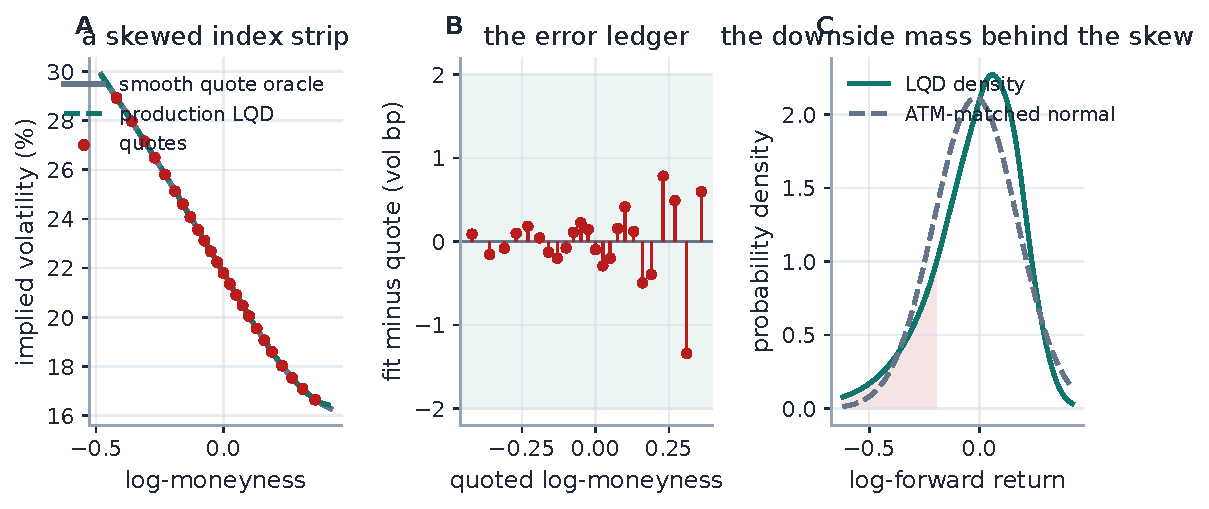
\includegraphics[width=\textwidth]{fig_lqd_fresh_spx.pdf}
\caption{The SPX-like case.  Panel A: quote oracle, quotes, and the
production fit.  Panel B: the error ledger at the quotes --- every residual
inside $\pm2$ vol bp (shaded), maximum \lqdfreshspxmaxerr\ vol bp against
quotes carrying a deliberate $\sim2$ bp ripple.  Panel C: the fitted density
against an ATM-matched normal: the entire content of the skew is the
transfer of mass into the left tail (shaded), bought by a thinner right
shoulder.  Beyond the quoted window the curve is the model's own
Lee-consistent extrapolation, not an oracle continuation.}
\label{fig:spx}
\end{figure}

\begin{figure}[H]
\centering
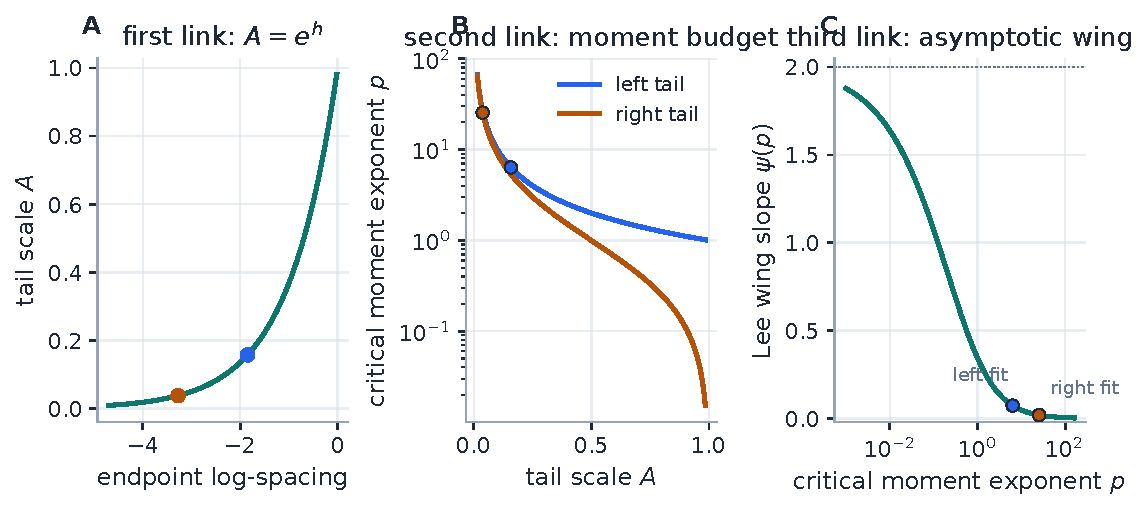
\includegraphics[width=\textwidth]{fig_lqd_fresh_tails.pdf}
\caption{The fitted tails walked through the three links of
\cref{sec:tails}: endpoint value of $g$ to tail scale ($A_L=\lqdfreshspxAL$,
$A_R=\lqdfreshspxAR$), tail scale to last finite moment
\eqref{eq:critical}, and moment to Lee wing slope \eqref{eq:lee_slopes}
($\beta_L=\lqdfreshspxbetaL$, $\beta_R=\lqdfreshspxbetaR$).  Nothing imposed
these wings; they are what the quoted body implied through the basis.}
\label{fig:spxtails}
\end{figure}

\subsection{Case file: the density wears two hats}
\label{sec:case_event}

Ahead of a scheduled binary event --- earnings, a court ruling, a
referendum --- the terminal density can be \emph{bimodal}: the market prices
two distinct landing zones.  A low-order direct-volatility model fights this
shape; a quadratic-in-$k$ smile cannot make a central trough with supported
wings.  The target here is an asymmetric mixture of two log-return normals
(weights $\lqdfresheventweightleft\%/44\%$, centres
$\lqdfresheventmeanleft$ and $+\lqdfresheventmeanright$ after martingale
normalization, distinct widths; \cref{app:oracles}) at
$\tau=24/365$, quoted at \lqdfresheventnquotes\ strikes.  A
$\lqdfresheventorder$-mode fit --- the top of the schema range, an event
slice's natural habitat --- recovers both the smile and the two-humped
density (\cref{fig:event}) with maximum error \lqdfresheventmaxerr\ vol bp,
endpoint scales $A_L=\lqdfresheventAL$, $A_R=\lqdfresheventAR$, and
$\E[e^{X}]-1=\lqdfresheventmart$.  Positivity of the density is automatic
even where the high Legendre modes carve the trough; what the basis
\emph{cannot} do is place an exact atom --- the hats are smooth by
construction (\cref{sec:limits}).  In a sparse live market one would lean on
the ridge or fix the handles through the chart of \cref{sec:ortho} to keep
the extra modes from fitting noise.

\begin{figure}[H]
\centering
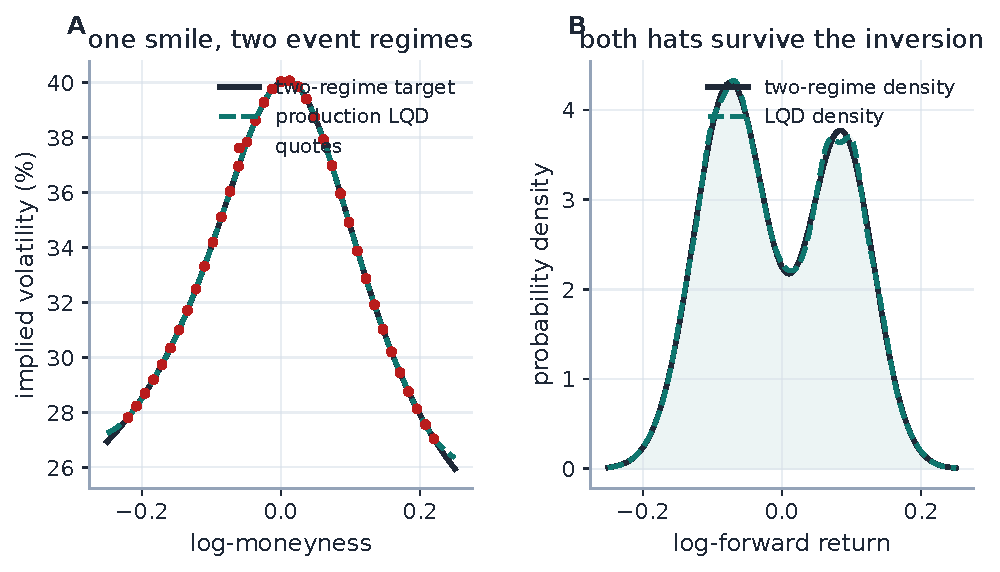
\includegraphics[width=\textwidth]{fig_lqd_fresh_event.pdf}
\caption{The event case.  Panel A: the two-regime target smile and the
$\lqdfresheventorder$-mode production fit --- note the W-shaped body a
low-order model cannot make.  Panel B: the true mixture density and the LQD
density: both hats, the asymmetry, and the trough survive the round trip
through option prices, with positivity never at risk.}
\label{fig:event}
\end{figure}

%======================================================================
\section{What is genuinely original here}
\label{sec:original}

Quantile-based and density-based smile constructions are not new, and the
Lee analysis is classical.  Three things in this implementation are worth
singling out:
\begin{enumerate}[leftmargin=1.6em]
\item \textbf{The endpoint basis} $-\log u-\log(1-u)+(1-u)L+uR$.  It makes
the tails exponential \emph{with controllable scale} while keeping the body
in a clean orthogonal-polynomial space; the Lee slopes
\eqref{eq:lee_slopes} then fall out of the parametrization instead of being
patched on.
\item \textbf{The exact ATM handles and the orthogonal chart}
(\cref{sec:handles}).  Level, skew and curvature are closed-form functionals
of the quantile, so the model carries genuine trader coordinates \emph{and}
a chart in which shape modes do not disturb them --- the same three handles
the graph extrapolator of Note~14 propagates.
\item \textbf{The implicit-root cancellation} (\cref{thm:cancel}).  The
strike root's dependence on $\theta$ vanishing from the price gradient turns
a $(P{+}1)$-rebuild finite-difference Jacobian into a one-pass analytic one,
audited to $\lqdfreshjacmaxrel$ column-wise against central differences.
\end{enumerate}

%======================================================================
\section{Limitations}
\label{sec:limits}

A lecture that sells a model without drawing its boundary is an
advertisement.  Here is where this one's guarantees stop.  The headline
first: LQD removes butterfly arbitrage by construction but \emph{not}
calendar arbitrage across independently fitted expiries --- the coupling of
\cref{sec:calendar} is soft, finite-weight and optional, so a coupled
surface is calendar-\emph{controlled}, not calendar-guaranteed.  Beyond
that:
\begin{itemize}[leftmargin=1.4em]
\item \textbf{Near the integrability wall.}  As $A_R\to1$ the forward
integral degenerates: the tail corrections \eqref{eq:tail_corr} dominate,
conditioning of the fit and of the retarget Newton solve deteriorates, and
the barrier is doing real work.  Admissible is not the same as comfortable.
\item \textbf{Atoms of any kind.}  The model is a continuous law on
$(0,\infty)$: not only a jump-to-default atom at zero but \emph{any} exact
mass point (a pinned settlement price, a tender offer) can only be
approximated by a sharp continuous feature, never represented.
\item \textbf{Positive is not plausible.}  Structural positivity guarantees
a \emph{density}, not a sensible one: an unregularized high-order fit can
produce economically implausible --- multi-modal, spiky --- yet perfectly
arbitrage-free shapes.  Positivity removes one failure class; the ridge,
band weighting and judgment handle the rest.
\item \textbf{Coefficient non-uniqueness in practice.}  Distinct coefficient
vectors can price indistinguishably (near-degenerate directions grow with
$N$ and with sparse data), so fitted coefficients are not comparable across
fits --- compare handles, curves and densities, not raw $\theta$.
\item \textbf{Unstudied sensitivities.}  There is no dedicated study of
handle \emph{drift} under rolling recalibration, nor of digital/one-touch
sensitivities to the interpolation scheme; both are open measurement items,
not established properties.
\end{itemize}

%======================================================================
\section{Traceability}
\label{sec:traceability}

One caveat on the ``match note'' anchors: the fixture coefficients those
tests lock were recorded when the original benchmark was frozen, so they are
\emph{legacy locks} --- they pin production behaviour against regression,
but their literal values can lag the freshly regenerated numbers in this
note (which always come from fresh generator runs).  Where the two disagree,
the fresh run is the current truth and the test is the regression tripwire.

\begingroup
\small
\setlength{\tabcolsep}{4pt}
\renewcommand{\arraystretch}{1.15}
\begin{longtable}{@{}p{0.30\textwidth}p{0.11\textwidth}p{0.55\textwidth}@{}}
\caption{Claims in this note and the code/tests that lock them.}\\
\toprule Claim & Object & Code anchor \newline \emph{Test anchors}\\ \midrule
\endfirsthead
\toprule Claim & Object & Code anchor \newline \emph{Test anchors}\\ \midrule
\endhead
Density positive; call curve monotone and convex; parity holds &
\cref{prop:nobutterfly} &
\nolinkurl{models/lqd/quadrature.py}\newline
\nolinkurl{test_lqd_pricing.py::test_density_positive}\newline
\nolinkurl{::test_call_curve_monotone_and_convex_in_strike}\newline
\nolinkurl{::test_put_call_parity}\\
\addlinespace
Martingale shift correct; $\E[e^X]=1$ &
\eqref{eq:mu_norm} &
\nolinkurl{models/lqd/quadrature.py}\newline
\nolinkurl{test_lqd_pricing.py::test_svi_fit_martingale_shift_matches_note}\newline
\nolinkurl{::test_svi_fit_martingale_integral_is_one}\\
\addlinespace
Endpoint scales and Lee slopes; stable for extreme scales &
\eqref{eq:endpoint_scales}--\eqref{eq:lee_slopes} &
\nolinkurl{models/lqd/basis.py}\newline
\nolinkurl{test_lqd_basis.py::test_svi_fit_endpoint_scales_match_note}\newline
\nolinkurl{::test_svi_fit_lee_slopes_match_note}\newline
\nolinkurl{::test_lee_slopes_stable_for_tiny_nonzero_endpoint_scales}\\
\addlinespace
Legendre basis: recursion and orthogonality &
\eqref{eq:leg_recursion} &
\nolinkurl{models/lqd/basis.py}\newline
\nolinkurl{test_lqd_basis.py::test_legendre_recursion_matches_explicit_polynomials}\newline
\nolinkurl{::test_legendre_orthogonality_on_unit_interval}\\
\addlinespace
Exact ATM handles &
\eqref{eq:atm_handles} &
\nolinkurl{models/lqd/atm.py}\newline
\nolinkurl{test_lqd_atm.py::test_atm_level_matches_implied_vol}\newline
\nolinkurl{::test_atm_skew_matches_finite_difference}\newline
\nolinkurl{::test_atm_curvature_matches_finite_difference}\\
\addlinespace
Orthogonal chart: shape moves preserve handles; retarget exact &
\cref{sec:ortho} &
\nolinkurl{models/lqd/ortho.py}\newline
\nolinkurl{test_lqd_ortho.py::test_shape_move_leaves_handles_nearly_unchanged}\newline
\nolinkurl{::test_retarget_hits_exact_handles}\\
\addlinespace
Analytic Jacobian matches FD (mid, band, calendar); fits agree &
\cref{thm:cancel} &
\nolinkurl{models/lqd/jacobian.py}\newline
\nolinkurl{test_lqd_jacobian.py::test_jacobian_matches_fd_mid}\newline
\nolinkurl{::test_jacobian_matches_fd_band}\newline
\nolinkurl{::test_jacobian_matches_fd_calendar}\newline
\nolinkurl{::test_analytic_and_fd_fits_agree}\\
\addlinespace
Barrier finite for wild trial parameters &
\eqref{eq:barrier} &
\nolinkurl{models/lqd/calibrate.py}\newline
\nolinkurl{test_lqd_jacobian.py::test_barrier_residual_finite_for_wild_tail_scale}\\
\addlinespace
Benchmark fit and speed rail (legacy fixture) &
\cref{sec:cases} &
\nolinkurl{models/lqd/calibrate.py}\newline
\nolinkurl{test_lqd_calibrate.py::test_calibrate_to_svi_benchmark}\newline
\nolinkurl{::test_calibration_is_fast_enough}\\
\addlinespace
Double-hat event smile: bimodal density recovered &
\cref{sec:case_event} &
\nolinkurl{models/lqd/calibrate.py}\newline
\nolinkurl{test_lqd_pricing.py::test_double_hat_density_is_bimodal}\\
\addlinespace
Calendar floor exact at constraint $z$-values &
\eqref{eq:calendar} &
\nolinkurl{calib/calendar.py}\newline
\nolinkurl{test_lqd_jacobian.py::test_jacobian_matches_fd_calendar}\\
\bottomrule
\end{longtable}
\endgroup

\appendix
%======================================================================
\section{LQD-native controls and numerical constants}
\label{app:atlas}

The knobs \emph{specific to} the LQD slice, with defaults and roles.
Surfaced knobs are user-facing \texttt{FitSettings}; hidden knobs are
internal constants tuned to the algorithm and not exposed.  The \emph{shared}
calibration controls that also shape an LQD fit --- \texttt{fitMode},
\texttt{haircut}, \texttt{midAnchorWeight},
\texttt{enforceCalendar}/\texttt{calendarWeight}, the var-swap controls, and
the prior-persistence and observation-filter settings of \cref{tab:stack}
--- are indexed in Note~00's control table and derived in their own notes
(07, 08, 10, 13, 15); they are deliberately not duplicated here.

\begin{longtable}{p{0.26\textwidth}p{0.12\textwidth}p{0.54\textwidth}}
\caption{LQD-native controls.}\label{tab:atlas}\\
\toprule
Knob & Default & Role\\
\midrule
\endfirsthead
\toprule Knob & Default & Role\\ \midrule
\endhead
\multicolumn{3}{l}{\emph{Surfaced (FitSettings)}}\\
\midrule
\texttt{nOrder} $N$ & $6$ & Legendre expansion order; $7$ parameters at
$N=6$.  Schema range $4\le N\le16$: $6$ for ordinary slices, $8$--$14$ for
scheduled-event slices.\\
\texttt{regLambda} $\lambda$ & $10^{-6}$ & High-order ridge coefficient in
\eqref{eq:calib_objective}; suppresses oscillation in sparse data.\\
\texttt{regPower} $r$ & $1.0$ & Ridge exponent in $n^{2r}a_n^2$; larger $r$
penalizes high modes harder.\\
\texttt{barrierCenter} $c$ & \lqdbarriercenter & Centre of the $A_R$ softplus
barrier \eqref{eq:barrier}; engages before the $A_R=1$ wall.\\
\texttt{barrierScale} $\gamma$ & \lqdbarrierscale & Steepness of that
barrier.\\
\texttt{weightScheme} & \texttt{equal} & Per-quote weighting of the data
residuals (\texttt{equal} or \texttt{tv\_density}); see Note~07.\\
\midrule
\multicolumn{3}{l}{\emph{Hidden (internal constants)}}\\
\midrule
\texttt{Z\_MAX} $Z$ & $40.0$ & Half-width of the symmetric log-odds grid;
truncation error $\ll$ vega noise for equity tails.\\
\texttt{N\_POINTS} & $8001$ & Reporting/diagnostic grid nodes (odd, so $z=0$
is a node).\\
\texttt{OPT\_N\_POINTS} & \lqdoptpts & Coarser grid used during optimization
iterations; the accepted slice is rebuilt at \texttt{N\_POINTS}.\\
\texttt{EPS\_AR} $\eps_R$ & $10^{-6}$ & Buffer in the hard bound
$A_R<1-\eps_R$.\\
\texttt{\_VEGA\_FLOOR} $\eta$ & $10^{-4}$ & Floor added to Black vega in the
residual normalization \eqref{eq:vega_resid}.\\
\texttt{xtol/ftol/gtol} & $10^{-10}$ & \texttt{trf} tolerances; $\sim6$
orders below the fit budget, so the optimum is display-identical while
\texttt{trf} stops grinding invisible reductions.\\
\texttt{max\_nfev} & $4000$ & Evaluation cap (rarely approached).\\
\bottomrule
\end{longtable}

%======================================================================
\section{Performance notes}
\label{app:perf}

\begin{enumerate}[leftmargin=1.6em]
\item \textbf{Cached static grid.}  The grid $(z,u,u(1-u))$ and the Legendre
matrix depend only on $(Z,n_{\text{pts}},N)$, so they are LRU-cached and
returned read-only; only $g$ is re-formed per call.  This removed
$\sim40\%$ of \texttt{build\_slice} and made each build $\sim1.7\times$
faster.
\item \textbf{Two-grid optimization.}  Iterations run on
\texttt{OPT\_N\_POINTS} $=\lqdoptpts$ (Simpson error already far below the
fit budget); the accepted slice is rebuilt once at $8001$ nodes for the
reported result and diagnostics.  Converged parameters agree with a
full-grid fit to $\sim10^{-6}$.
\item \textbf{Hermite interpolation/inversion.}  Storing the exact nodal
derivatives $\dd Q/\dd z$ and $\dd G/\dd z$ gives cubic-Hermite off-grid
evaluation (clean Greeks) and machine-precision strike inversion by
Hermite--Newton --- and supplies precisely the nodal sensitivities the
analytic Jacobian reuses.
\item \textbf{Analytic Jacobian} (\cref{sec:jacobian}).  One quadrature pass
instead of $P+1$ finite-difference rebuilds, reaching the same fitted
solution within tolerance (relative cost agreement $\sim10^{-11}$), measured
$1.3$--$1.7\times$ on the residual-path benchmark of \cref{tab:timing} and
structurally more on heavier configurations.  Gated to the
var-swap/prior-free configuration.
\item \textbf{Looser tolerances.}  Dropping \texttt{trf} tolerances from
$10^{-15}$ to $10^{-10}$ stops the optimizer chasing cost reductions
invisible in the priced surface, saving whole $(P{+}1)$-evaluation
iterations at no display-precision cost.
\end{enumerate}

%======================================================================
\section{The synthetic oracles}
\label{app:oracles}

The case files fit production against two deterministic quote oracles;
neither is used anywhere inside the model.

\paragraph{The SSVI-shaped strip.}  The SPX-like target is the total-variance
curve
\begin{equation}
w(k)=\frac{\vartheta}{2}\Big(1+\rho\phi k
+\sqrt{(\phi k+\rho)^{2}+1-\rho^{2}}\Big),
\qquad
(\vartheta,\rho,\phi)=(0.0356,\,-0.68,\,2.40),
\end{equation}
Gatheral--Jacquier's SSVI slice shape \cite{GatheralJacquier2014},
sampled at the \lqdfreshspxnquotes\ strikes listed in the generator and
perturbed by the deterministic ripple
$10^{-4}(1.20\sin(9k+0.4)+0.55\cos(21k))$ in volatility.  (The regression
fixture behind the legacy timing table, \cref{tab:timing}, is the older
five-parameter raw-SVI benchmark; the JW re-coordinatization used to specify
it is Note~02's subject.)

\paragraph{The two-regime mixture.}  The event target is an equal-mean
mixture of two log-return normals with weights
$(\lqdfresheventweightleft\%,44\%)$, raw centres $(-0.075,+0.085)$ shifted by
a common constant so the mixture is a martingale, and widths
$(0.052,0.047)$.  Its normalized calls are the exact two-term Gaussian
formula
\begin{equation}
C(k)=\sum_{i}w_i\Big(
e^{m_i+\sigma_i^{2}/2}\,
\PhiN\!\Big(\tfrac{m_i+\sigma_i^{2}-k}{\sigma_i}\Big)
-e^{k}\,\PhiN\!\Big(\tfrac{m_i-k}{\sigma_i}\Big)\Big),
\end{equation}
inverted to implied volatilities for quoting.  This oracle has genuinely
bimodal density, which is the point.

%======================================================================
\section{Reference implementation}
\label{app:ref}

The whole slice is one quadrature pass in the log-odds coordinate: form $g$,
integrate $\dd Q/\dd z=e^{g}$ to the quantile, solve one scalar
normalization for the martingale shift $\mu$, reverse-integrate the upper
share $G$, and price every strike by \eqref{eq:call_price}.  Executed
against production before committing: the listing reproduces
\texttt{build\_slice}'s quantile and share to $10^{-12}$ and $\mu$ to
$10^{-14}$ on an $N=6$ slice, and returns $\E[e^{X}]=1.000000$ (production
inverts $Q(z_k)=k$ by Hermite--Newton and interpolates $G$ with cubic
Hermite for smooth Greeks; the linear \texttt{np.interp} here prices calls
to $\sim10^{-6}$ on the dense grid).

\begin{lstlisting}[caption={The LQD quadrature pipeline (distilled from
\texttt{models/lqd/\{basis,quadrature\}.py}).}]
def legendre(n_max, x):            # P_0..P_{n_max}, 3-term recursion
    P = np.empty((n_max+1, x.size)); P[0] = 1.0; P[1] = x
    for n in range(1, n_max):
        P[n+1] = ((2*n+1)*x*P[n] - n*P[n-1]) / (n+1)
    return P

def g_of_u(u, L, R, a):            # smooth part g(u) of log q(u)
    return (1-u)*L + u*R + a @ legendre(len(a)+1, 1 - 2*u)[2:]

def build_slice(z, L, R, a):
    # One quadrature pass, eqs (Q_of_z)-(upper_share).
    u = expit(z); dz = z[1] - z[0]
    # Tail scales e^{g(0)}, e^{g(1)}:
    A_L, A_R = np.exp(g_of_u(np.array([0.0, 1.0]), L, R, a))
    dQ = np.exp(g_of_u(u, L, R, a))          # dQ/dz = e^{g}
    Q = cumulative_simpson(dQ, dx=dz, initial=0.0)
    Q -= Q[len(z)//2]                        # anchor Q(0) = 0
    mass = np.exp(Q)*u*(1-u)
    tot = (np.trapezoid(mass, z)             # + analytic tails
           + np.exp(Q[-1]-z[-1])/(1-A_R)
           + np.exp(Q[0]-z[-1])/(1+A_L))
    mu = -np.log(tot); Q = Q + mu            # now E[e^X] = 1
    m = np.exp(Q)*u*(1-u)
    # Upper share G(z) = int_z^inf e^{Q} u(1-u):
    G = (cumulative_simpson(m[::-1], dx=dz, initial=0.0)[::-1]
         + np.exp(Q[-1]-z[-1])/(1-A_R))
    return u, Q, G

def call_price(k, z, u, Q, G):
    # C(k) = G(z_k) - e^k (1 - u_k)
    zk = np.interp(k, Q, z)                  # invert Q(z_k) = k
    return np.interp(zk, z, G) - np.exp(k)*(1 - expit(zk))
\end{lstlisting}

\begin{thebibliography}{9}
\bibitem{BreedenLitzenberger1978} D.~Breeden and R.~Litzenberger.
Prices of state-contingent claims implicit in option prices.
\emph{Journal of Business}, 51(4):621--651, 1978.
\bibitem{Lee2004} R.~W.~Lee.
The moment formula for implied volatility at extreme strikes.
\emph{Mathematical Finance}, 14(3):469--480, 2004.
\bibitem{Gatheral2006} J.~Gatheral.
\emph{The Volatility Surface: A Practitioner's Guide}. Wiley, 2006.
\bibitem{GatheralJacquier2014} J.~Gatheral and A.~Jacquier.
Arbitrage-free SVI volatility surfaces.
\emph{Quantitative Finance}, 14(1):59--71, 2014.
\bibitem{Strassen1965} V.~Strassen.
The existence of probability measures with given marginals.
\emph{Annals of Mathematical Statistics}, 36(2):423--439, 1965.
\bibitem{CarrMadan1998} P.~Carr and D.~Madan.
Towards a theory of volatility trading.
In \emph{Volatility}, Risk Books, 1998.
\end{thebibliography}

\end{document}
